\documentclass[draft]{agujournal2019}
\usepackage{url} %this package should fix any errors with URLs in refs.
\usepackage{lineno}
%\usepackage[inline]{trackchanges} %for better track changes. finalnew option will compile document with changes incorporated.
\usepackage{soul}
\linenumbers

\usepackage{xr}
\externaldocument{si_rev1}

\draftfalse

\journalname{JGR: Atmospheres}

\begin{document}

\title{Ship-based lidar evaluation of Southern Ocean low clouds in the storm-resolving general circulation model ICON and the ERA5 and MERRA-2 reanalyses}

\authors{Peter Kuma\affil{1,2,3,4}, Frida A.-M. Bender\affil{1,2}, Adrian J. McDonald\affil{3}, Simon P. Alexander\affil{5,6}, Greg M. McFarquhar\affil{7,8}, John J. Cassano\affil{9,10,11}, Graeme E. Plank\affil{3}, Sean Hartery\affil{3}\thanks{Current affiliation: Department of Physics \& Atmospheric Science, Dalhousie University, Halifax, Canada}, Simon Parsons\affil{3}\thanks{Current affiliation: New South Wales Department of Planning and Environment, Sydney, New South Wales, Australia}, Sally Garrett\affil{12}, Alex J. Schuddeboom\affil{3}, and Anna Possner\affil{4}}

\affiliation{1}{Department of Meteorology (MISU), Stockholm University, Stockholm, Sweden}
\affiliation{2}{Bolin Centre for Climate Research, Stockholm University, Stockholm, Sweden}
\affiliation{3}{School of Physical and Chemical Sciences, University of Canterbury, Christchurch, Aotearoa/New Zealand}
\affiliation{4}{Institute for Atmospheric and Environmental Sciences, Goethe University Frankfurt, Frankfurt am Main, Hesse, Germany}
\affiliation{5}{Australian Antarctic Division, Kingston, Tasmania, Australia}
\affiliation{6}{Australian Antarctic Program Partnership, Institute for Marine and Antarctic Studies, University of Tasmania, Hobart, Tasmania, Australia}
\affiliation{7}{Cooperative Institute of Severe and High Impact Weather Research and Operations, University of Oklahoma, Norman, OK, USA}
\affiliation{8}{School of Meteorology, University of Oklahoma, Norman, OK, USA}
\affiliation{9}{Cooperative Institute for Research in Environmental Sciences, University of Colorado, Boulder, CO, USA}
\affiliation{10}{National Snow and Ice Data Center, University of Colorado, Boulder, CO, USA}
\affiliation{11}{Department of Atmospheric and Oceanic Sciences, University of Colorado, Boulder, CO, USA}
\affiliation{12}{New Zealand Defence Force, Wellington, Aotearoa/New Zealand}

\correspondingauthor{Peter Kuma}{peter@peterkuma.net}

\begin{keypoints}
\item Large cloud biases are present in the global storm-resolving model, but are lower in several key aspects than in the reanalyses.
\item The models tend to underestimate total cloud fraction, near-surface cloud and fog, while overestimating cloud occurrence peak at 500 m.
\item A ``too few, too bright'' problem of underestimated cloud fraction, compensated by overestimated cloud albedo, is present in MERRA-2.
\end{keypoints}

\begin{abstract}
Global storm resolving models (GSRMs) represent the next generation of global climate models. One of them is a 5-km Icosahedral Nonhydrostatic Weather and Climate Model (ICON). Its high resolution means that parameterizations of convection and clouds, including subgrid-scale clouds, are omitted, relying on explicit simulation but necessarily utilizing microphysics and turbulence parameterizations. Standard-resolution (10--100~km) models, which use convection and cloud parameterizations, have substantial cloud biases over the Southern Ocean (SO), adversely affecting radiation and sea surface temperature. The SO is dominated by low clouds, which cannot be observed accurately from space due to overlapping clouds, attenuation, and ground clutter. We evaluated SO clouds in ICON and the ERA5 and MERRA-2 reanalyses using approximately 2400 days of lidar observations and 2300 radiosonde profiles from 31 voyages and Macquarie Island station during 2010--2021, compared with the models using a ground-based lidar simulator. We found that ICON and the reanalyses underestimate the total cloud fraction by about 10 and 20\%, respectively. ICON and ERA5 overestimate the cloud occurrence peak at about 500~m, associated with underestimated lower tropospheric stability and overestimated lifting condensation level. The reanalyses strongly underestimate fog and near-surface clouds, and MERRA-2 underestimates cloud occurrence at almost all heights. Outgoing shortwave radiation is overestimated in MERRA-2, implying a ``too few, too bright'' cloud problem. SO cloud and fog biases are a substantial issue in the analyzed models and result in shortwave and longwave radiation biases.
\end{abstract}

\section*{Plain Language Summary}

Global storm-resolving models are climate models with km-scale horizontal resolution, which are currently in development. Reanalyses are the best estimates of past meteorological conditions based on an underlying global model and observations. We evaluated clouds, temperature, and humidity profiles over the Southern Ocean in one such model, as well as two reanalyses, based on 2400 days of ship and station observations. Thanks to the high resolution, the model relies entirely on explicit simulation of clouds instead of subgrid-scale parameterizations. For the evaluation, we used ceilometer and radiosonde observations and a lidar simulator, which enables a fair comparison with the model and reanalyses. We subsetted our results by cyclonic activity and stability. We found that the model and reanalyses underestimate lidar-derived cloud fraction, and the reanalyses do so more strongly. Fog or near-surface clouds are especially underestimated in the reanalyses. However, the model and one of the reanalyses also tend to overestimate the peak of cloud occurrence at 500 m above the ground, and it tends to be higher. This is linked to thermodynamic profiles, which show a higher lifting condensation level and lower stability. Southern Ocean cloud and fog biases are an important problem in the analyzed models and result in radiation balance biases.

\section{Introduction}
\label{sec:introduction}

Increasing climate model spatial resolution is one way of improving the accuracy of the representation of the climate system in models \cite{mauritsen2022}. It has been practiced since the advent of climate modeling as more computational power, memory, and storage capacity become available. It is, however, often not as easy as changing the grid size because of the complex interplay between model dynamics and physics, which necessitates adjusting and tuning all components together. Increasing resolution is, of course, limited by the available computational power and a trade-off with increasing parameterization complexity, which is another way of improving model accuracy. Current computational availability and acceleration from general-purpose computing on graphics processing units (GPUs) has progressed to enable km-scale (also called k-scale) Earth system models (ESMs) and coupled atmosphere--ocean general circulation models (AOGCMs) for research today and will become operational in the future. Therefore, it represents a natural advance in climate modeling. Global storm-resolving models (GSRMs) are emerging as a new front in the development of high-resolution global climate models, with horizontal grid resolutions of about 2--8~km \cite{satoh2019,stevens2019}. This resolution is enough to resolve mesoscale convective storms, but smaller-scale convective plumes and cloud structure remain unresolved. At an approximately 5-km scale, non-hydrostatic processes also become important \cite{weisman1997}, and for this reason such models are generally non-hydrostatic. The terms global cloud-resolving models or global convection-permitting/-resolving models are also sometimes used interchangeably with GSRMs but imply that clouds or convection are resolved explicitly, which is not entirely true for GSRMs, as this would require an even higher horizontal resolution \cite{satoh2019}. Representative of these efforts is the DYnamics of the Atmospheric general circulation Modeled On Non-hydrostatic Domains (DYAMOND) project \cite{stevens2019,dyamond}, which is an intercomparison of nine global GSRMs over two 40-day time periods in summer (1~August--10~September 2016) and winter (20~January--1~March 2020). A new one-year GSRM intercomparison is currently proposed by \citeA{takasuka2024}, with the hope of also evaluating the seasonal cycle and large-scale circulation. An alternative to using a computationally costly GSRM is to train an artificial neural network on GSRM output and use it for subgrid-scale clouds, as done with the GSRM ICON by \citeA{grundner2022} and \citeA{grundner2023}.

The main aim of this study is to evaluate the GSRM version of ICON developed by the nextGEMS project \cite{nextgems,segura2025}. ICON is developed and maintained jointly by Deutscher Wetterdienst, the Max-Planck-Institute for Meteorology, Deutsches Klimarechenzentrum (DKRZ), Karlsruhe Institute of Technology, and the Center for Climate Systems Modeling. Our aim is to quantify how well the GSRM ICON simulates clouds in this region, particularly in light of the fact that subgrid-scale clouds and convection are not parameterized in this model. This region is mostly dominated by boundary layer clouds generated by shallow convection, and these are problematic to observe by spaceborne lidars and radars, which are affected by attenuation by overlapping and thick clouds \cite{mace2009,medeiros2010} and ground clutter \cite{marchand2008}, respectively. Specifically, the radar on CloudSat and lidar on the Cloud-Aerosol Lidar and Infrared Pathfinder Satellite Observation (CALIPSO), neither of which are now operational, are affected by the above-mentioned issues, resulting in a strong underestimation of cloud occurrence below 2 km in a merged CloudSat--CALIPSO product relative to ground-based lidar observations at McMurdo Station \cite{mcerlich2021}. However, removing situations with higher overlapping clouds could enable a less biased comparison of low clouds. We hypothesize that this, in turn, can lead to systematic biases in low clouds in climate models, which are frequently evaluated against CloudSat--CALIPSO products. Reanalyses can also suffer from cloud biases, as these are usually parameterized in their atmospheric component and also in regions where input observations are sparse. This makes them a problematic reference for clouds over the SO, and any biases relative to a reanalysis should be interpreted with caution. Instead, we chose to use a large set of ship-based observations conducted with ceilometers and lidars on board the RV \emph{Polarstern} and other voyages and a station as a reference for the model evaluation. Altogether, we analyzed approximately 2400 days of data from 31 voyages and one sub-Antarctic station covering diverse longitudes and latitudes of the SO. To achieve a like-for-like comparison with the model, we used a ground-based lidar simulator called the Automatic Lidar and Ceilometer Framework [ALCF; \citeA{kuma2021}]. We contrasted the results with ERA5 \cite{era5} and the Modern-Era Retrospective analysis for Research and Applications, Version~2 [MERRA-2; \citeA{gelaro2017}].

The nextGEMS project focuses on the research and development of GSRMs at multiple modeling centers and universities in Europe. The project also develops GSRM versions of the Icosahedral Nonhydrostatic Weather and Climate Model (ICON; \citeA{hohenegger2023}), the Integrated Forecasting System [IFS; \citeA{ifs2023}], and their ocean components at eddy-resolving resolutions: ICON-O \cite{korn2022} coupled with ICON and Finite-Element/volumE Sea ice-Ocean Model [FESOM; \citeA{wang2014a}] and Nucleus for European modeling of the Ocean [NEMO; \citeA{madec2023}] coupled with IFS. The project has so far produced ICON and IFS simulations with three development versions called Cycle 1--3 and a pre-final version, with a final production version planned by the end of the project. nextGEMS is not the only project developing GSRMs; other GSRMs (or GSRM versions of climate models) currently in development include: Convection-Permitting Simulations With the E3SM Global Atmosphere Model [SCREAM; \citeA{caldwell2021}], Non-hydrostatic Icosahedral Atmospheric Model [NICAM; \citeA{satoh2008}], Unified Model (UM), eXperimental System for High-resolution modeling for Earth-to-Local Domain [X-SHiELD; \citeA{shield}], Action de Recherche Petite Echelle Grande Echelle-NonHydrostatic version [ARPEGE-NH; \citeA{bubnova1995,voldoire2017}], Finite-Volume Dynamical Core on the Cubed Sphere [FV3, \citeA{lin2004}], the National Aeronautics and Space Administration (NASA) Goddard Earth Observing System global atmospheric model version 5 [GEOS5; \citeA{putman2011}], Model for Prediction Across Scales [MPAS; \citeA{skamarock2012}], and System for Atmospheric Modeling [SAM; \citeA{khairoutdinov2003}].

Multiple cloud properties have an effect on shortwave (SW) and longwave (LW) radiation. To first order, the total cloud fraction, cloud phase, and the liquid and ice water path are the most important cloud properties influencing SW and LW radiation. These properties are in turn influenced by the atmospheric thermodynamics, convection and circulation, and both the indirect and direct effects of aerosols. Second-order effects on SW and LW radiation are associated with the cloud droplet size distribution, ice crystal habit, cloud lifetime, and direct radiative interaction with aerosols. In the 6$^\mathrm{th}$ phase of the Coupled Model Intercomparison Project [CMIP6; \citeA{eyring2016}], the cloud feedback has increased relative to CMIP5 \cite{zelinka2020}, especially in the Southern Hemisphere mid-to-high latitudes, which is one of the main reasons for the higher climate sensitivity of CMIP6 models.

The Southern Ocean (SO) is known to be a problematic region for climate model biases \cite{schuddeboom2021,hyder2018,cesana2022,zhao2022} due to a lack of surface and in situ observations and being a lower priority region for numerical weather prediction (NWP) and climate model development because of its distance from populated areas. Nevertheless, radiation biases and changes over an area of its size have a substantial influence on the global climate \cite{rintoul2011}, such as affecting the Earth's radiation balance, ocean heat, and carbon uptake \cite{williams2023}, and the SO is also an important part of the global ocean conveyor belt \cite{wang2014b}. In general, marine clouds have a disproportionate effect on top-of-atmosphere (TOA) SW radiation due to the relatively low albedo of the sea surface. The relative longitudinal symmetry of the SO means that model cloud biases tend to be similar across longitudes.

In the following text, we refer to the SO as ocean regions south of 40°S, low-latitude SO as 40--55°S, and high-latitude SO as south of 55°S, all the way to the Antarctic coast. The reason for this dividing latitude is to split the SO into about two equal zones, as well as the results by \citeA{schuddeboom2021} (Fig.~2b) which show a contrast in CMIP model radiation biases. \citeA{schuddeboom2019} (Fig.~2) and \citeA{kuma2020} (Fig.~3) also show contrasting radiation biases in the Hadley Centre Global Environmental Model, which is also supported by \citeA{cesana2022}, displaying contrasting cloud biases due to the 0°C isotherm reaching the surface at 55°S. The findings of \citeA{niu2024}, however, support a different dividing line of 62°S based on cloud condensation nuclei concentration.

SO radiation biases have been relatively large and systematic compared to the rest of the globe since at least CMIP3 \cite{trenberth2010}, and the SO SW cloud radiative effect (CRE) bias is still positive in eight CMIP6 models analyzed by \citeA{schuddeboom2021} over the high-latitude SO, whereas over the low-latitude SO it tends to be more neutral or negative in some models. Too much absorbed SW radiation over the SO was also identified in the GSRM SCREAM \cite{caldwell2021}. Compensating biases are possible, such as the ``too few too bright'' cloud bias, characterized by too small a cloud fraction and too large a cloud albedo \cite{wall2017,kuma2020}, previously described by \citeA{webb2001}, \citeA{weare2004}, \citeA{zhang2005}, \citeA{karlsson2008}, \citeA{nam2012}, \citeA{klein2013}, and \citeA{bender2017} in other regions and models, which means that a model can maintain a reasonable SW radiation balance by reflecting too much SW radiation from clouds, but these cover too small an area. A study by \citeA{konsta2022} showed that this type of bias is still present in six analyzed CMIP6 models in tropical marine clouds, using the GCM-Oriented CALIPSO Cloud Product [CALIPSO--GOCCP; \citeA{chepfer2010}] and Polarization \& Anisotropy of Reflectances for Atmospheric Sciences coupled with Observations from a Lidar [PARASOL; \citeA{lier2008}] as a reference. They suggest improper simulation of subgrid-scale cloud heterogeneity as a cause. Compensating cloud biases in the Australian Community Climate and Earth System Simulator (ACCESS) – Atmosphere-only model version 2 (AM2) over the SO were analyzed by \citeA{fiddes2022} and \citeA{fiddes2024}. \citeA{possner2022} showed that over the SO, the DYAMOND GSRM ICON underestimates low-level cloud fraction on the order of 30\% and overestimates net downward TOA SW radiation by approximately 10 Wm$^\mathrm{-2}$ in the highest model resolution run (2.5~km). \citeA{zhao2022} reported a similar SW radiation bias in five analyzed CMIP6 models over the high-latitude SO and an underestimation of the total cloud fraction on the order of 10\% over the entire 40--60°S SO. Recently, \citeA{ramadoss2024} analyzed 48~hours of km-scale ICON limited-area model NWP simulations over an SO region adjacent to Tasmania against the Clouds, Aerosols, Precipitation, Radiation, and atmospherIc Composition Over the southeRn oceaN (CAPRICORN) voyage cloud and precipitation observations \cite{mcfarquhar2021}. They found the ICON cloud optical thickness was underestimated relative to Himawari‐8 satellite observations but also identified large differences in cloud top phase.

In general, sea surface temperature (SST) biases in the SO can originate either in the atmosphere \cite{hyder2018}, caused by too much shortwave heating of the surface or too little longwave cooling of the surface, such as in situations of too much cloud cover or cloud optical thickness, or in the ocean circulation. Interactions of both are also possible; for example, SST affecting clouds and clouds affecting the surface radiation. Using the European Centre for Medium-Range Weather Forecasts (ECMWF) Reanalysis 5 (ERA5) as a reference, \citeA{zhang2023} have shown that SST biases have improved in CMIP6 compared to CMIP5, with SST overall increasing in CMIP6. However, over the SO, this resulted in an even higher positive bias, especially in the Atlantic Ocean (AO) sector of the SO, increasing by up to 1°C. \citeA{luo2023} identified that the SO SST bias in an ensemble of 18 CMIP6 models originates not from the surface heat and radiation fluxes (using reanalyses as a reference) but from a warm bias in the Northern Atlantic Deep Water.

\begin{figure}[b!]
\centering
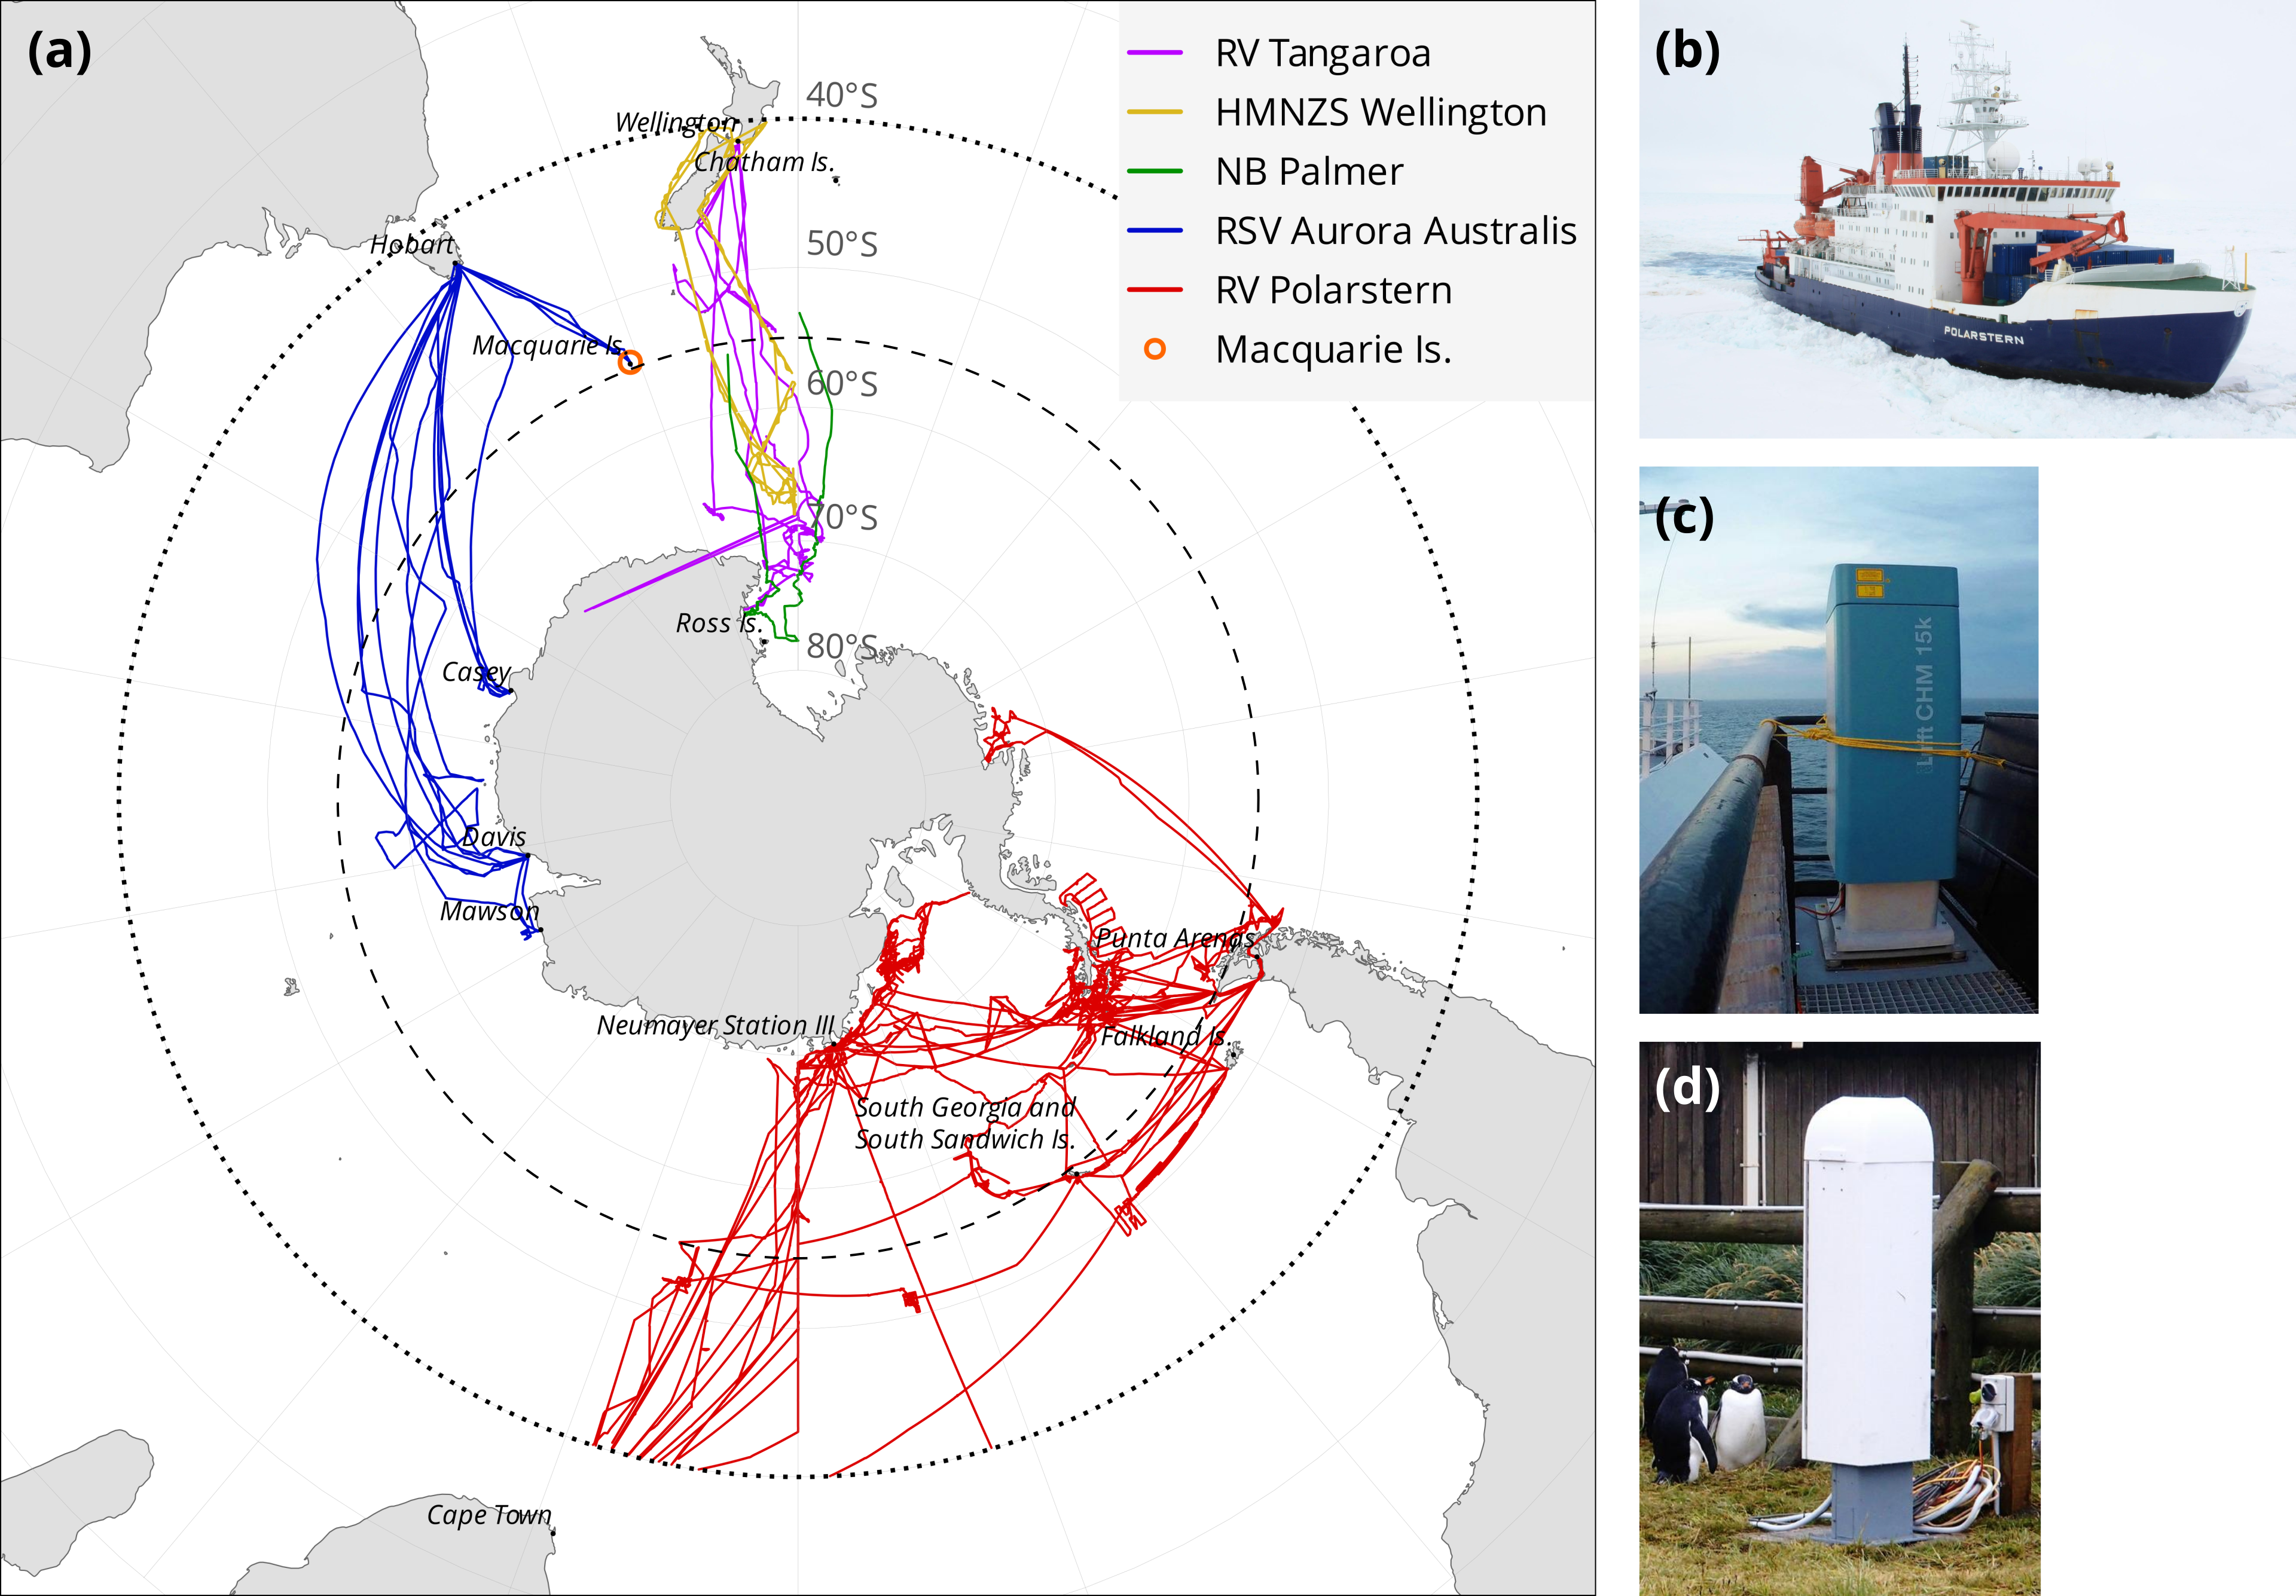
\includegraphics[width=\textwidth]{img/map_fig.pdf}
\caption{
\textbf{(a)} A map showing the tracks of 31 voyages of RV \emph{Polarstern}, RSV \emph{Aurora Australis}, RV \emph{Tangaroa}, RV \emph{Nathaniel B. Palmer}, and HMNZS \emph{Wellington} and one sub-Antarctic station (Macquarie Island) analyzed here. The tracks cover Antarctic sectors south of South America, the Atlantic Ocean, Africa, Australia, and New Zealand in the years 2010--2021 (inclusive). The dotted and dashed lines at 40°S and 55°S delineate the Southern Ocean area of our analysis and its partitioning into two subsets, respectively. A photo of \textbf{(b)} RV \emph{Polarstern} (© Folke Mehrtens, Alfred-Wegener-Institut), \textbf{(c)} Lufft CHM~15k installed on RV \emph{Tangaroa} (© Peter Kuma, University of Canterbury), \textbf{(d)} Vaisala CL51 (© Jeff Aquilina, Bureau of Meteorology), \textbf{(e)} Vaisala CT25K at Macquarie Island (© Simon P.\ Alexander, Australian Antarctic Division).
}
\label{fig:map}
\end{figure}

\section{Methods}
\label{sec:methods}

\subsection{Voyage and Station Data}

Together, we analyzed data from 31 voyages of RV \emph{Polarstern}, the resupply vessel (RSV) \emph{Aurora Australis}, RV \emph{Tangaroa}, RV \emph{Nathaniel B. Palmer}, Her (now His) Majesty's New Zealand Ship (HMNZS) \emph{Wellington}, and one sub-Antarctic station (Macquarie Island) in the SO south of 40°S between 2010 and 2021. Fig.~\ref{fig:map} shows a map of the campaigns, Table \ref{tab:voyages} lists the campaigns, and Table \ref{tab:voyage-references} lists references where available. The analyzed dataset comprised 2421 days of data south of 40°S, but the availability of ceilometer data was slightly shorter due to gaps in measurements.

The campaigns contained ceilometer observations captured by the Vaisala CL51, CT25K, and the Lufft CHM~15k, described in detail below (Sections~\ref{sec:cl51} and \ref{sec:chm15k}). A ceilometer is a low-power, near-infrared, vertically pointing lidar principally designed to measure cloud base, but they also measure the full vertical structure of clouds as long as the laser signal is not attenuated by thick clouds, which can be used to infer additional information such as a cloud mask and cloud occurrence by height. We note that during the MICRE campaign, the ceilometers Vaisala CT25K and CL51 were installed at the Macquarie Island station concurrently, but in our analysis we only used the CT25K data obtained from the Atmospheric Radiation Measurement (ARM) data archive.

Apart from lidar observations, radiosondes were launched on weather balloons at regular synoptic times on the RV \emph{Polarstern}, MARCUS, NBP17024, TAN1702, and TAN1802 campaigns, measuring pressure, temperature, relative humidity, and the global navigation satellite system coordinates. Derived thermodynamic (virtual potential temperature, relative humidity, lifting condensation level, etc.) and dynamic physical quantities (wind speed and direction) for the measured vertical profiles were calculated with the program radiosonde tool [rstool; \citeA{rstool}]. Surface meteorological quantities were measured continuously by an onboard automatic weather station or individual instruments.

Some of the observatial data were likely used in reanalysis assimilation. The Macquarie Island station surface measurements and radiosonde profiles (not used in our analysis), were sent to the World Meteorological Organization Global Telecommunication System (GTS). The lidar measurements and radiosonde profiles on the RSV \textit{Aurora Australis} were not sent for assimilation.

\begin{table}[p!]
\caption{
An overview of the analyzed campaigns (voyages and stations). Start, end, and the number of days (UTC; inclusive) refer to the time period when the vessel was south of 40°S. Abbreviations: ceilometer (ceil.), Australia (AU), New Zealand (NZ), South America (SA), Atlantic Ocean (AO), and Africa (AF). The number of days is rounded to the nearest integer. CL51/31 indicates CL51 configured to emulate CL31. Missing days in the ceilometer data were HMNZSW16 (7 days): 24--27 November, 10~December, 16--17~December 2016; MARCUS (3 days): 8, 10~November, 10~December 2017; MICRE (9~days): 7--8, 29~June, 5, 16~July, 15~August, 17~October 2016, 11~February, 21~March 2017; TAN1502 (1~day): 24~January.
}
\label{tab:voyages}
\centering
\small
\begin{tabular}{llllllr}
\textbf{Name} & \textbf{Vessel or station} & \textbf{Ceil.} & \textbf{Region} & \textbf{Start} & \textbf{End} & \textbf{Days}\\
\hline
AA15-16  & RSV \emph{Aurora Australis}   & CL51    & AU       & 2015-10-22 & 2016-02-22 & 124 \\
HMNZSW16 & HMNZS \emph{Wellington}       & CHM 15k & NZ       & 2016-11-23 & 2016-12-19 & 27 \\
MARCUS   & RSV \emph{Aurora Australis}   & CT25K   & AU       & 2017-10-29 & 2018-03-26 & 149 \\
MICRE    & Macquarie Is. station         & CT25K   & AU/NZ    & 2016-04-03 & 2018-03-14 & 710 \\
NBP1704  & RV \emph{Nathaniel B. Palmer} & CHM 15k & NZ       & 2017-04-14 & 2017-06-08 & 55 \\
PS77/2   & RV \emph{Polarstern}          & CL51    & SA/AO/AF & 2010-12-01 & 2011-02-04 & 65 \\
PS77/3   & RV \emph{Polarstern}          & CL51    & SA/AO/AF & 2011-02-07 & 2011-04-14 & 66 \\
PS79/2   & RV \emph{Polarstern}          & CL51    & SA/AO/AF & 2011-12-06 & 2012-01-02 & 27 \\
PS79/3   & RV \emph{Polarstern}          & CL51    & SA/AO/AF & 2012-01-10 & 2012-03-10 & 61 \\
PS79/4   & RV \emph{Polarstern}          & CL51    & SA/AO/AF & 2012-03-14 & 2012-04-08 & 26 \\
PS81/2   & RV \emph{Polarstern}          & CL51    & SA/AO/AF & 2012-12-02 & 2013-01-18 & 47 \\
PS81/3   & RV \emph{Polarstern}          & CL51    & SA/AO/AF & 2013-01-22 & 2013-03-17 & 55 \\
PS81/4   & RV \emph{Polarstern}          & CL51    & SA/AO/AF & 2013-03-18 & 2013-04-16 & 30 \\
PS81/5   & RV \emph{Polarstern}          & CL51    & SA/AO/AF & 2013-04-20 & 2013-05-23 & 33 \\
PS81/6   & RV \emph{Polarstern}          & CL51    & SA/AO/AF & 2013-06-10 & 2013-08-12 & 63 \\
PS81/7   & RV \emph{Polarstern}          & CL51    & SA/AO/AF & 2013-08-15 & 2013-10-14 & 60 \\
PS81/8   & RV \emph{Polarstern}          & CL51    & SA/AO/AF & 2013-11-12 & 2013-12-14 & 31 \\
PS81/9   & RV \emph{Polarstern}          & CL51    & SA/AO/AF & 2013-12-21 & 2014-03-02 & 71 \\
PS89     & RV \emph{Polarstern}          & CL51    & SA/AO/AF & 2014-12-05 & 2015-01-30 & 56 \\
PS96     & RV \emph{Polarstern}          & CL51    & SA/AO/AF & 2015-12-08 & 2016-02-14 & 68 \\
PS97     & RV \emph{Polarstern}          & CL51    & SA/AO/AF & 2016-02-15 & 2016-04-06 & 52 \\
PS103    & RV \emph{Polarstern}          & CL51    & SA/AO/AF & 2016-12-18 & 2017-02-02 & 46 \\
PS104    & RV \emph{Polarstern}          & CL51    & SA/AO/AF & 2017-02-08 & 2017-03-18 & 39 \\
PS111    & RV \emph{Polarstern}          & CL51    & SA/AO/AF & 2018-01-21 & 2018-03-14 & 52 \\
PS112    & RV \emph{Polarstern}          & CL51    & SA/AO/AF & 2018-03-18 & 2018-05-05 & 49 \\
PS117    & RV \emph{Polarstern}          & CL51    & SA/AO/AF & 2018-12-18 & 2019-02-07 & 51 \\
PS118    & RV \emph{Polarstern}          & CL51    & SA/AO/AF & 2019-02-18 & 2019-04-08 & 50 \\
PS123    & RV \emph{Polarstern}          & CL51    & SA/AO/AF & 2021-01-10 & 2021-01-31 & 21 \\
PS124    & RV \emph{Polarstern}          & CL51    & SA/AO/AF & 2021-02-03 & 2021-03-30 & 55 \\
TAN1502  & RV \emph{Tangaroa}            & CL51/31 & NZ       & 2015-01-20 & 2015-03-12 & 51 \\
TAN1702  & RV \emph{Tangaroa}            & CHM 15k & NZ       & 2017-03-09 & 2017-03-31 & 23 \\
TAN1802  & RV \emph{Tangaroa}            & CHM 15k & NZ       & 2018-02-07 & 2018-03-20 & 41 \\
\hline
\textbf{Total} &                         &         &          &            &            & \textbf{2421}\\
\hline
\end{tabular}
\normalsize
\end{table}

\begin{table}[t!]
\caption{Campaign publication references.}
\label{tab:voyage-references}
\centering
\small
\begin{tabular}{lp{14.5cm}}
\textbf{Name} & \textbf{References}\\
\hline
AA15-16  & \citeA{klekociuk2020} \\
MARCUS   & \citeA{mcfarquhar2021,xia2024,niu2024} \\
MICRE    & \citeA{mcfarquhar2021} \\
NBP1704  & \citeA{ackley2020} \\
PS77/2   & \citeA{kniglanglo2011a,kniglanglo2011b,kniglanglo2011c,kniglanglo2014a,fahrbach2011} \\
PS77/3   & \citeA{kniglanglo2011d,kniglanglo2011e,kniglanglo2012a,kniglanglo2014b,knust2011} \\
PS79/2   & \citeA{kniglanglo2012b,kniglanglo2012c,kniglanglo2012d,kniglanglo2014c,kattner2012} \\
PS79/3   & \citeA{kniglanglo2012e,kniglanglo2012f,kniglanglo2012g,kniglanglo2014d,wolfgladrow2012} \\
PS79/4   & \citeA{kniglanglo2012h,kniglanglo2012i,kniglanglo2012j,kniglanglo2014e,lucassen2012} \\
PS81/2   & \citeA{kniglanglo2013a,kniglanglo2013b,kniglanglo2013c,kniglanglo2014f,boebel2013} \\
PS81/3   & \citeA{kniglanglo2013d,kniglanglo2013e,kniglanglo2013f,kniglanglo2014g,gutt2013} \\
PS81/4   & \citeA{kniglanglo2013g,kniglanglo2013h,kniglanglo2013i,kniglanglo2014q,bohrmann2013} \\
PS81/5   & \citeA{kniglanglo2013j,kniglanglo2013k,kniglanglo2013l,kniglanglo2014r,jokat2013} \\
PS81/6   & \citeA{kniglanglo2013m,kniglanglo2013n,kniglanglo2013o,kniglanglo2014h,lemke2013} \\
PS81/7   & \citeA{kniglanglo2013p,kniglanglo2013q,kniglanglo2014i,kniglanglo2016a,meyer2013} \\
PS81/8   & \citeA{kniglanglo2013r,kniglanglo2014j,kniglanglo2014k,kniglanglo2014l,schlindwein2014} \\
PS81/9   & \citeA{kniglanglo2014m,kniglanglo2014n,kniglanglo2014o,kniglanglo2014p,knust2014} \\
PS89     & \citeA{kniglanglo2015a,kniglanglo2015b,kniglanglo2015c,kniglanglo2015d,boebel2016}\\
PS96     & \citeA{kniglanglo2016b,kniglanglo2016c,kniglanglo2016d,kniglanglo2016e,schrder2017} \\
PS97     & \citeA{kniglanglo2016f,kniglanglo2016g,kniglanglo2016h,kniglanglo2016i,lamy2017} \\
PS103    & \citeA{kniglanglo2017a,kniglanglo2017b,kniglanglo2017c,kniglanglo2017d,boebel2018} \\
PS104    & \citeA{kniglanglo2017e,kniglanglo2017f,kniglanglo2017g,gohl2018,schmithsen2021a} \\
PS111    & \citeA{schmithsen2019a,schmithsen2020a,schmithsen2021b,schmithsen2021c,schrder2018} \\
PS112    & \citeA{schmithsen2019b,schmithsen2020b,schmithsen2021d,schmithsen2021e,meyer2018} \\
PS117    & \citeA{schmithsen2019c,schmithsen2020c,schmithsen2021f,schmithsen2021g,boebel2019} \\
PS118    & \citeA{schmithsen2019d,schmithsen2020d,schmithsen2021h,schmithsen2021i,dorschel2019} \\
PS123    & \citeA{schmithsen2021j,schmithsen2021m,schmithsen2021n,schmithsen2021k,hoppmann2023a} \\
PS124    & \citeA{schmithsen2021o,schmithsen2021q,schmithsen2021p,hoppmann2023b} \\
TAN1802  & \citeA{kremser2020,kremser2021} \\
\hline
\end{tabular}
\end{table}

\subsection{Vaisala CL51 and CT25K}
\label{sec:cl51}

The Vaisala CL51 and CT25K (photos in Fig.~\ref{fig:map}d, e) are ceilometers operating at near-infrared wavelengths of 910~nm and 905~nm, respectively. The CL51 can also be configured to emulate the Vaisala CL31. The maximum range is 15.4~km (CL51), 7.7~km (CL31 emulation mode with 5~m vertical resolution), and 7.5~km (CT25K). The vertical resolution is 10~m (5~m configurable) in CL51 and 30~m in CT25K observations. The sampling (temporal) resolution is configurable, and in our datasets, it is approximately 6~s for CL51 on AA15‐16, 16~s for CT25K on MARCUS and MICRE, 36~s for CL51 on RV \emph{Polarstern}, and about 2.37~s for CL51 with CL31 emulation on TAN1502. The wavelengths of 905 and 910~nm are both affected by water vapor absorption of about 20\% in the mid-latitudes \cite{wiegner2015,wiegner2019}, with 910~nm affected more strongly, but we do not expect this to be a significant issue, as explained in \citeA{kuma2021}. The instrument data files containing raw uncalibrated backscatter were first converted to Network Common Data Form (NetCDF) with cl2nc \cite{kuma2024a} and then processed with the ALCF (Section~\ref{sec:alcf}) to produce absolutely calibrated attenuated volume backscattering coefficient (AVBC), cloud mask, cloud occurrence by height, and the total cloud fraction. Because the CT25K uses a very similar wavelength to the CL51, equivalent calculations as for the CL51 were done assuming a wavelength of 910~nm. The Vaisala CL51 and CT25K instruments were used on most of the voyages and stations analyzed here. Fig.~\ref{fig:example}a shows an example of AVBC derived from the CL51 instrument data.

\begin{figure}[b!]
\centering
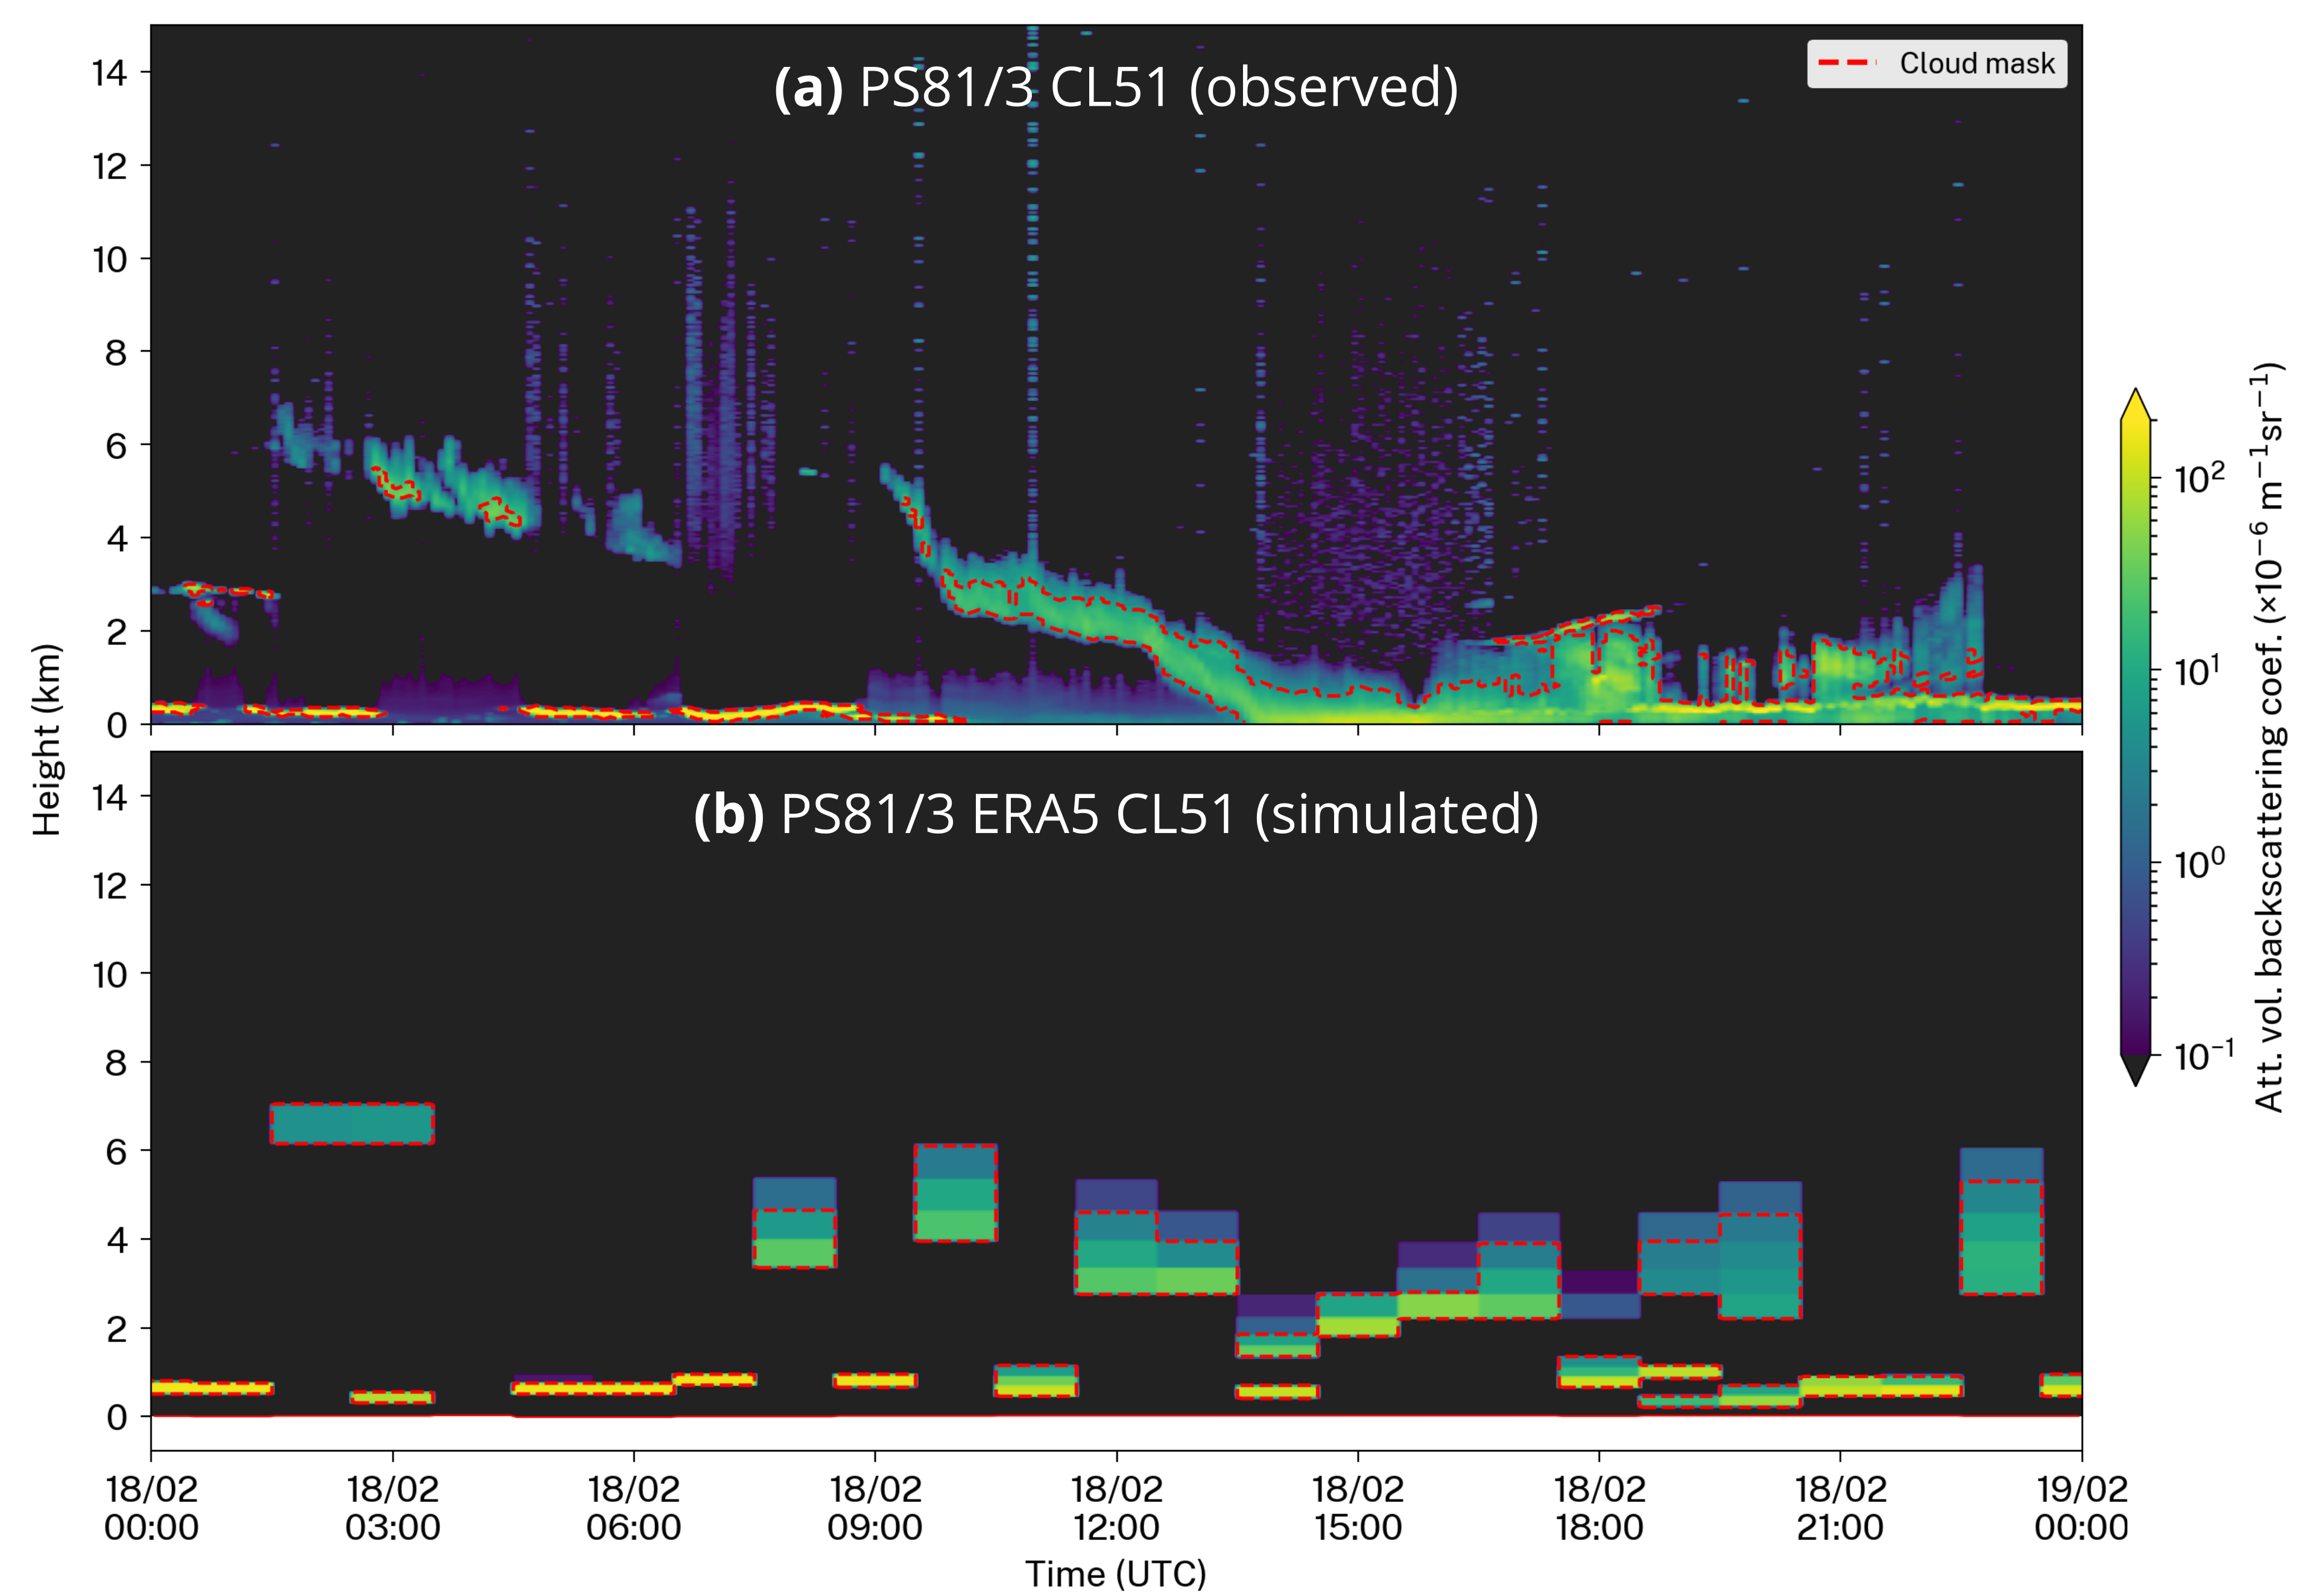
\includegraphics[width=\textwidth]{img/example.png}
\caption{
An example of the attenuated volume backscattering coefficient (AVBC) \textbf{(a)} measured by the CL51 during 24~hours on the PS81/3 voyage and \textbf{(b)} an equivalent AVBC simulated with the ALCF from ERA5 data during the same time period. The red line identifies the cloud mask determined by the ALCF.
}
\label{fig:example}
\end{figure}

\subsection{Lufft CHM~15k}
\label{sec:chm15k}

The Lufft CHM~15k (photo in Fig.~\ref{fig:map}c) ceilometer operates at a near-infrared wavelength of 1064~nm. The maximum range is 15.4~km; the vertical resolution is 5~m in the near range (up to 150~m) and 15~m above; the sampling (temporal) resolution is 2~s; and the number of vertical levels is 1024. NetCDF files containing uncalibrated backscatter produced by the instrument were processed with the ALCF (Section~\ref{sec:alcf}) to again produce AVBC, cloud mask, cloud occurrence by height, and the total cloud fraction. The CHM~15k was used on four voyages (HMNZSW16, TAN1702, TAN1802, and NBP1704).

\subsection{ALCF}
\label{sec:alcf}

The Automatic Lidar and Ceilometer Framework (ALCF) is a ground-based lidar simulator and a tool for processing observed lidar data, supporting various instruments and models \cite{kuma2021}. It performs radiative transfer calculations to derive equivalent lidar AVBC from an atmospheric model, which can then be compared with observed AVBC. For this purpose, it takes the cloud fraction, liquid and ice mass mixing ratio, temperature, and pressure model fields as an input and is run offline (on the model output rather than inside the model code). The lidar simulator in the ALCF is based on the instrument simulator Cloud Feedback Model Intercomparison Project (CFMIP) Observation Simulator Package (COSP) \cite{bodas-salcedo2011}. After AVBC is calculated, a cloud mask, cloud occurrence by height, and the total cloud fraction are determined. The total cloud fraction is defined as the fraction of profiles with clouds at any height in the lidar cloud mask. The ALCF has been used by several research teams for model and reanalysis evaluation \cite{kuma2020,kremser2021,guyot2022,pei2023,whitehead2023,mcdonald2024a}.

Absolute calibration of the observed backscatter was performed by comparing the measured clear-sky molecular backscatter statistically with simulated clear-sky molecular backscatter. AVBC was resampled to 5 min temporal resolution and 50~m vertical resolution to increase the signal-to-noise ratio while having enough resolution to detect small-scale cloud variability. The noise standard deviation was calculated from AVBC at the highest range, where no clouds are expected. A cloud mask was calculated from AVBC using a fixed threshold of $\mathrm{2\times 10^{-6} m^{-1}sr^{-1}}$ after subtracting 5 standard deviations of range-scaled noise. Fig.~\ref{fig:example}b shows an example of simulated Vaisala CL51 backscatter from ERA5 data, corresponding to a day of measurements by the instrument on the PS81/3 voyage.

How attenuation of the lidar signal affects cloud detection is dependent on factors such as the optical thickness of the measured cloud and its backscattering phase function, as well as the range-dependent noise standard deviation. A rough estimate can be made under an assumption of a relatively strongly backscattering cloud of $\beta = \mathrm{100\times 10^{-6} m^{-1}sr^{-1}}$ at a height of $r_1$ = 2 km, range-dependent noise $\beta_n$ at $r_2$ = 8 km of about $\mathrm{5\times 10^{-6} m^{-1}sr^{-1}}$, and cloud detection threshold $\beta_t = \mathrm{2\times 10^{-6} m^{-1}sr^{-1}}$, noise multiplication factor $f$ = 5, at full attenuation the two-way attenuation factor $A$ satisfies $A\beta = \beta_t + f\times \beta_n\left(\frac{r_1}{r_2}\right)^2$, which is equivalent to exponential decay ($A = e^{-2\delta}$) with optical depth $\delta$ (at the lidar wavelength) of about 1.7.

\subsection{ICON}
\label{sec:icon}

A coupled (atmosphere--ocean) GSRM version of the ICON model is in development as part of the nextGEMS project \cite{hohenegger2023}. ICON is a very flexible model, allowing for simulations ranging from coarse-resolution ESM simulations, GSRM simulations, limited area model simulations, and large eddy simulations (LES) for both weather prediction and climate projections. ICON uses the atmospheric component ICON-A \cite{giorgetta2018}, whose physics is derived from ECHAM6 \cite{stevens2013}, and the ocean component ICON-O \cite{korn2022}. Earlier runs of the GSRM ICON from DYAMOND were evaluated by \citeA{mauritsen2022}.

Here, we use a free-running (i.e., the weather conditions in the model do not correspond to reality) coupled GSRM simulation made for the purpose of climate projection. nextGEMS has so far produced four cycles of model runs. We used a Cycle 3 run \emph{ngc3028} produced in 2023 \cite{nextgems2023a,nextgems2023b} for a model time period of 20 January 2020 to 22 July 2025, of which we analyzed the period 2021--2024 (inclusive). The horizontal resolution of ngc3028 is about 5 km. The model output is available on 90 vertical levels and 3-hourly instantaneous temporal resolution.

Unlike current general circulation models (GCMs), the storm-resolving version of ICON does not use convective and cloud parameterization but relies on explicit simulation of convection and clouds on the model grid. Subgrid-scale clouds are not resolved, and the grid cell cloud fraction is always either 0 or 100\%. While this makes the code development simpler without having to rely on uncertain parameterizations, it can miss smaller-scale clouds below the grid resolution. Turbulence and cloud microphysics have to be parameterized in this model as in other models, and aerosols are derived from a climatology. To account for the radiative effects of subgrid-scale clouds, a cloud inhomogeneity factor is introduced in the model, which scales down the cloud liquid water for radiative calculations. It ranges from 0.4 at lower tropospheric stability (LTS) of 0~K to 0.8 at 30~K. In addition, turbulent mixing in the Smagorinsky scheme was adjusted to allow mixing or entrainment in situations of no mixing under the traditional scheme, affecting stratocumulus clouds but not trade wind clouds \cite{segura2025}.

Because the analyzed ICON simulation was free-running (years 2021--2024, inclusive), weather and climate oscillations (such as the El Niño--Southern Oscillation phase) are not expected to be equivalent to reality at the same time and place. To compare with the observations collected during a different time period (years 2010--2021, inclusive), we compared the model output with observations at the same time of year and geographical location, as determined for each data point, such as a lidar profile or a radiosonde launch. In the ALCF, this was done using the \emph{override\_year} option (\url{https://alcf.peterkuma.net/documentation/cli/cmd_model.html}). For radiosonde profiles, the same mapping of time was done. That is, when selecting an equivalent profile from the model, the time of the profile was changed so that the time relative to the start of the year was preserved, but the year was changed to one of the four years available in the model data. Thus, for every radiosonde launch, there were four equivalent model profiles. The geographical location was kept the same.

Due to our comparison being long-term and large-scale, it is expected that a comparison between the free-running model and observations is statistically robust, despite weather-related differences between the two. Furthermore, the results from multiple campaigns are combined in a way that equal statistical weight is given to each campaign, eliminating an outsize influence of longer campaigns, allowing us to estimate uncertainty ranges under the assumption of independence of weather conditions between the campaigns, and ensuring that the results are statistically representative over the whole area covered by the campaigns. Different approaches to a comparison would be possible. For example, one could use only the first several days of a free-running simulation initialized from observations (or a reanalysis) for a comparison, as done in the Transpose-AMIP experiments \cite{williams2013}, thus being able to compare clouds and the physical drivers under the same weather conditions. Another possibility is the use of a model nudged to a reanalysis \cite{kuma2020}, but this was not available for our ICON simulations. We discuss further the implications of comparing the observations with a free-running model in Section~\ref{sec:limitations}.

\subsection{MERRA-2}

The Modern-Era Retrospective analysis for Research and Applications, Version 2 (MERRA-2) is a reanalysis produced by the Global Modeling and Assimilation Office at the NASA Goddard Space Flight Center \cite{gelaro2017}. It uses version 5.12.4 of the Goddard Earth Observing System (GEOS) atmospheric model \cite{rienecker2008,molod2015}. Non-convective clouds (condensation, autoconversion, and evaporation) are parameterized using a prognostic scheme \cite{bacmeister2006}, and sub-grid cloud fraction is determined using total water distribution and a critical relative humidity threshold. The reanalysis output analyzed here is available at a spatial resolution of 0.5° of latitude and 0.625° of longitude, which is about 56 km in the North--South direction and 35 km in the East--West direction at 60°S. The number of vertical model levels is 72. Here, we use the following products: 1-hourly instantaneous 2D single-level diagnostics (M2I1NXASM) for 2-m temperature and humidity; 3-hourly instantaneous 3D assimilated meteorological fields (M2I3NVASM) for cloud quantities, pressure, and temperature; 1-hourly average 2D surface flux diagnostics (M2T1NXFLX) for precipitation; and 1-hourly average 2D radiation diagnostics (M2T1NXRAD) for radiation quantities \cite{merra2}. Vertically resolved fields in M2I3NVASM start at a height of about 60 m, which limits our analysis of fog and near-surface clouds in this reanalysis.

\subsection{ERA5}

ERA5 \cite{era5} is a reanalysis produced by the ECMWF. It is based on a numerical weather prediction model IFS version CY41R2. It uses the \citeA{tiedtke1993} prognostic cloud scheme and \citeA{forbes2014} for mixed-phase clouds. The horizontal resolution is 0.25° in latitude and longitude, which is about 28~km in the North--South direction and 14~km in the East--West direction at 60°S. Internally, the model uses 137 vertical levels. Here, we use output at 1-hourly instantaneous time intervals, except for radiation quantities, which are accumulations (from these we calculate daily means). Vertically resolved quantities are made available on 37 pressure levels.

\subsection{CERES}
\label{sec:ceres}

TOA radiation quantities are taken from the CERES instruments onboard the Terra and Aqua satellites \cite{wielicki1996,loeb2018}. In our analysis, we used adjusted all-sky SW and LW upwelling fluxes at TOA, adjusted cloud liquid and ice water paths, and adjusted cloud amount from the synoptic TOA and surface fluxes and clouds 1-degree daily edition 4A product (CER\_SYN1deg-Day\_Terra-Aqua-MODIS\_Edition4A) \cite{doelling2013,doelling2016}. The water paths in the product are computed from optical depth and particle size from geostationary satellites and the Moderate Resolution Imaging Spectroradiometer [MODIS, \citeA{pagano1993}] \cite{ceres2025}. The water paths were multiplied by the cloud amount to get the water path relative to the whole grid cell area, equivalent to the definition used in the models.

Radiation and water path calculations presented in the results (Section~\ref{sec:results}) were completed such that they always represent daily means in order to be consistent with the CERES SYN1deg data. Therefore, every instantaneous profile in the simulated lidar data was assigned a daily mean radiation and water path value corresponding to the day (in the Coordinated Universal Time; UTC). In turn, the average radiation and water paths during the entire voyage or station observation period were calculated as averages of the profile values. In the observed lidar data, the daily mean values were taken from the spatially and temporally co-located CERES SYN1deg data for the day (in UTC). The voyage or station average was calculated in the same way.

\begin{figure}[b!]
\centering
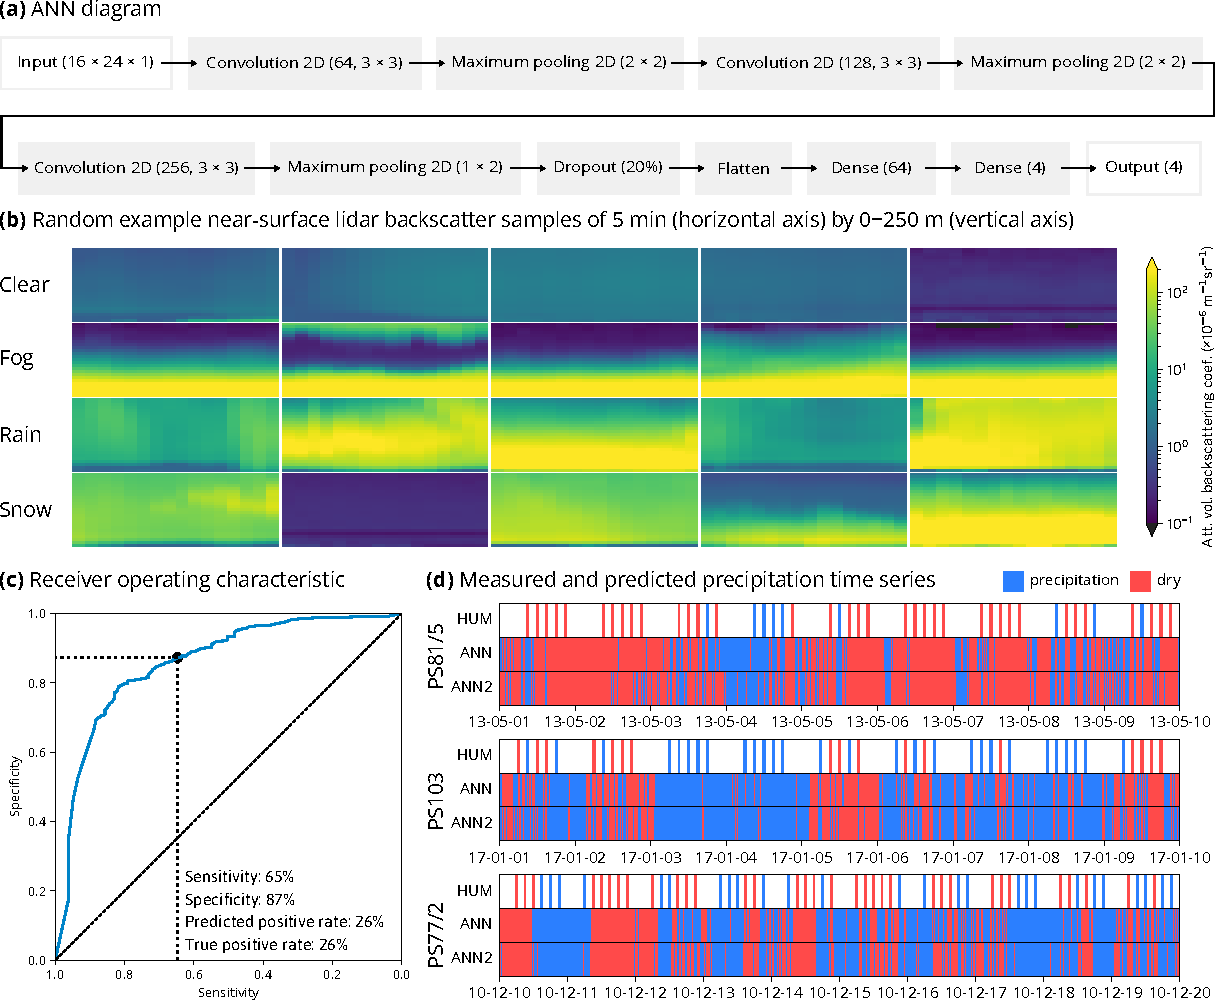
\includegraphics[width=\textwidth]{img/ann.pdf}
\caption{
Artificial neural network (ANN) for prediction of precipitation in lidar backscatter. \textbf{(a)} Diagram showing the TensorFlow structure of the ANN, \textbf{(b)} randomly selected example samples of near-surface backscatter in four categories (clear, fog, rain, and snow), as determined by coincident manual weather observations, \textbf{(c)} receiver operating characteristic diagram of the ANN, \textbf{(d)} examples of 10-day time series of human-observed (``HUM'') and predicted precipitation based on an ANN trained on all voyages (``ANN'') and all voyages except for the shown voyage (``ANN2'') during three randomly selected voyages with the available data. Here, by ``randomly selected,'' we mean selected from the top of a permutation generated by a pseudo-random number generator to prevent authors' bias in the selection.
}
\label{fig:ann}
\end{figure}

\subsection{Precipitation Identification Using Machine Learning}
\label{sec:ann}

Precipitation can cause strong enough lidar backscattering to be recognized as clouds by the threshold-based cloud detection method used in the ALCF. This is undesirable if equivalent precipitation backscatter is not included in the simulated lidar profiles. It was not possible to include precipitation simulation in the ALCF due to the absence of required fields of liquid and ice precipitation mass mixing ratios in the model output. While the fields could in principle be calculated from surface fluxes, such a calculation would be highly uncertain. The required radiation calculations for precipitation are also currently not implemented in the ALCF, even though this is a planned future addition. In order to achieve a fair comparison of observations with model output, we exclude observed and simulated lidar profiles with precipitation, either manually or using an automated method. It is relatively difficult to distinguish precipitation backscatter from cloud backscatter in lidar observations, especially when only one wavelength channel and no polarized channel are available \cite{kim2020}. In models, the same can be accomplished relatively easily by excluding profiles exceeding a certain surface precipitation flux. In the observations, using precipitation flux measurements from rain gauges can be very unreliable on ships due to ship movement, turbulence caused by nearby ship structures, and sea spray. Our analysis of rain gauge data from the RV \emph{Tangaroa} showed large discrepancies between the rain gauge time series and human-performed synoptic observations, as well as large inconsistencies in the rain gauge time series. Human-performed observations of precipitation presence or absence are expected to be reliable but only cover a limited set of times. Therefore, it was desirable to implement a method of detecting precipitation from observed backscatter profiles alone.

On the RV \emph{Polarstern} voyages, regular manual synoptic observations were available and included precipitation presence or absence and type. We used this dataset to train a convolutional artificial neural network (ANN) to recognize profiles with precipitation from lidar backscatter data (Fig.~\ref{fig:ann}a), implemented in the TensorFlow ANN framework \cite{tensorflow}. Samples of short time intervals (10~min) of near-surface lidar backscatter (0–250 m) were classified as clear, rain, snow, and fog, using the synoptic observations as a training dataset (Fig.~\ref{fig:ann}b). From these, a binary, mutually exclusive classification of profiles as precipitating (rain or snow) or dry (clear or fog) was derived. For detecting model and reanalysis precipitation, we used a fixed threshold for surface precipitation flux of 0.1 mm h$^{-1}$ (the ANN was not used).

The ANN achieved 65\% sensitivity and 87\% specificity when the true positive rate (26\%) was made to match observations. The receiver operating characteristic curve is shown in Fig.~\ref{fig:ann}c. We considered these rates satisfactory for the purpose of filtering precipitation profiles. Fig.~\ref{fig:ann}d shows examples of the predicted precipitation compared to human-performed observations. The main ANN (`ANN` in Fig.~\ref{fig:ann}) was trained on all data, and ancillary ANNs (`ANN2` in Fig.~\ref{fig:ann}) were trained with portions of voyage data excluded to test the results for each voyage.

\begin{figure}[b!]
\centering
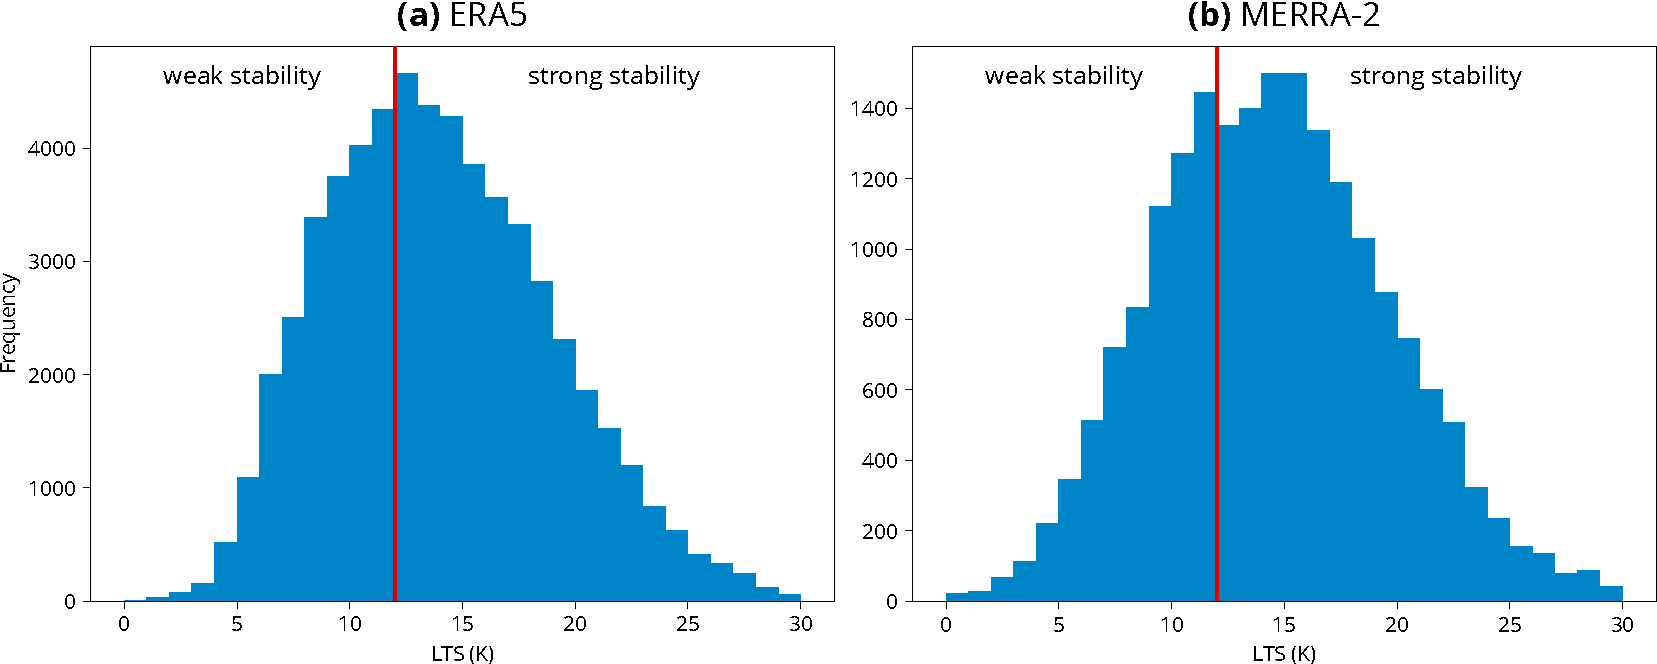
\includegraphics[width=\textwidth]{img/lts_dist.pdf}
\caption{
Lower tropospheric stability (LTS) distribution in \textbf{(a)} ERA5 and \textbf{(b)} MERRA-2 calculated for the 31 voyage tracks and one station from the highest instantaneous temporal resolution data available. Shown is also the chosen dividing threshold of 12 K for conditions of weak and strong stability.
}
\label{fig:lts}
\end{figure}

\subsection{Partitioning by Cyclonic Activity and Stability}
\label{sec:cyclone-stability}

In our analysis we partitioned our dataset by cyclonic activity and stability into multiple subsets in order to evaluate cloud biases in the context of the main physical controlling processes. The SO is a region of occurrence of both extratropical and polar cyclones. Cyclonic activity results in cloud formation at the air mass boundaries along the cold and warm fronts, as well as inside the cold sector, after a passing cold sector destabilizes the atmosphere relative to the surface temperature. In the cold front and cold sector, clouds are convectively driven, including deep convection, and the advection of colder air masses over warmer ocean surfaces can trigger convection and subsequent cloud formation. Conversely, warm advection can trigger fog or cloud formation by boundary layer air cooled by the ocean surface until it reaches saturation. More quiescent areas outside of cyclones can also be associated with clouds. These can be, for example, associated with clouds formed by warm or cold advection outside of cyclones, persistent clouds, clouds formed due to diurnal heating or cooling, or due to ocean currents. Boundary layer stability can be expected to be associated with clouds by either allowing convection and turbulence under weak stability, inhibiting convection turbulence under strong stability, and by capping inversion controlling the cloud top height or trapping moist air near the surface and preventing fog dispersion. Therefore, dividing our dataset by these subsets allows us to quantify model biases associated with some of the main physical processes controlling cloud formation, persistence, and dissipation. Other methods of subsetting, such as using the ISCCP pressure--optical thickness diagram \cite{rossow1991,rossow1999,hahn2001} to separate profiles by cloud regimes and other cloud regime classifications \cite{oreopoulos2016,schuddeboom2018}, would be feasible.

We partitioned our data into two mutually exclusive subsets by cyclonic activity. For this purpose, we used a cyclone tracking algorithm to identify extratropical and polar cyclones (ECs and PCs) over the SO in the reanalysis and ICON data. We used the open-source cyclone tracking package CyTRACK \cite{perez-alarcon2024}. Generally, what constitutes an EC is considered relatively arbitrary due to the very large variability of ECs \cite{neu2013}. The CyTRACK algorithm uses mean sea level pressure and wind speed thresholds as well as tracking across time steps to identify cyclone centers and their radii in each time step. With this information, we could classify every location at a given time as either cyclonic or non-cyclonic. Due to a relatively small total area covered by cyclones, as identified by the cyclone center and radius, for every time step and cyclone we defined a cyclonic area as a circle of double the radius identified by CyTRACK centered at the cyclone center. All other areas were defined as non-cyclonic. For identifying cyclones in the observations and the reanalyses, ERA5 pressure and wind fields were used as the input to CyTRACK. This is justified by the fact that the large-scale pressure and wind fields in ERA5 are likely sufficiently close to reality. \citeA{mcerlich2023} have shown that wind is simulated well in ERA5 relative to the WindSat polarimetric microwave radiometer measurements \cite{meissner2009}. For identifying cyclones in ICON, its own pressure and wind fields were used as the input to CyTRACK because the model is free-running, and thus the pressure and wind fields are different from reality. Subsetting by proximity to cyclones is a relatively crude measure because it does not take into account the different sectors of cyclones, which are commonly associated with different weather situations. However, this was a choice made for simplicity of the analysis, given the quantity of data. \citeA{konstali2024} performed a more complex attribution of precipitation to individual cyclone features.

In addition to the above, we partitioned our data into two mutually exclusive subsets based on LTS, which is derived as the difference between the potential temperature at 700~hPa and the surface. Based on a histogram of LTS in ERA5 and MERRA-2 calculated at all voyage tracks and stations (Fig.~\ref{fig:lts}), we determined a statistically based dividing threshold of 12~K for weak stability ($<$~12~K) and strong stability ($\geq$~12~K) conditions.

\section{Results}
\label{sec:results}

\begin{figure}[p!]
\centering
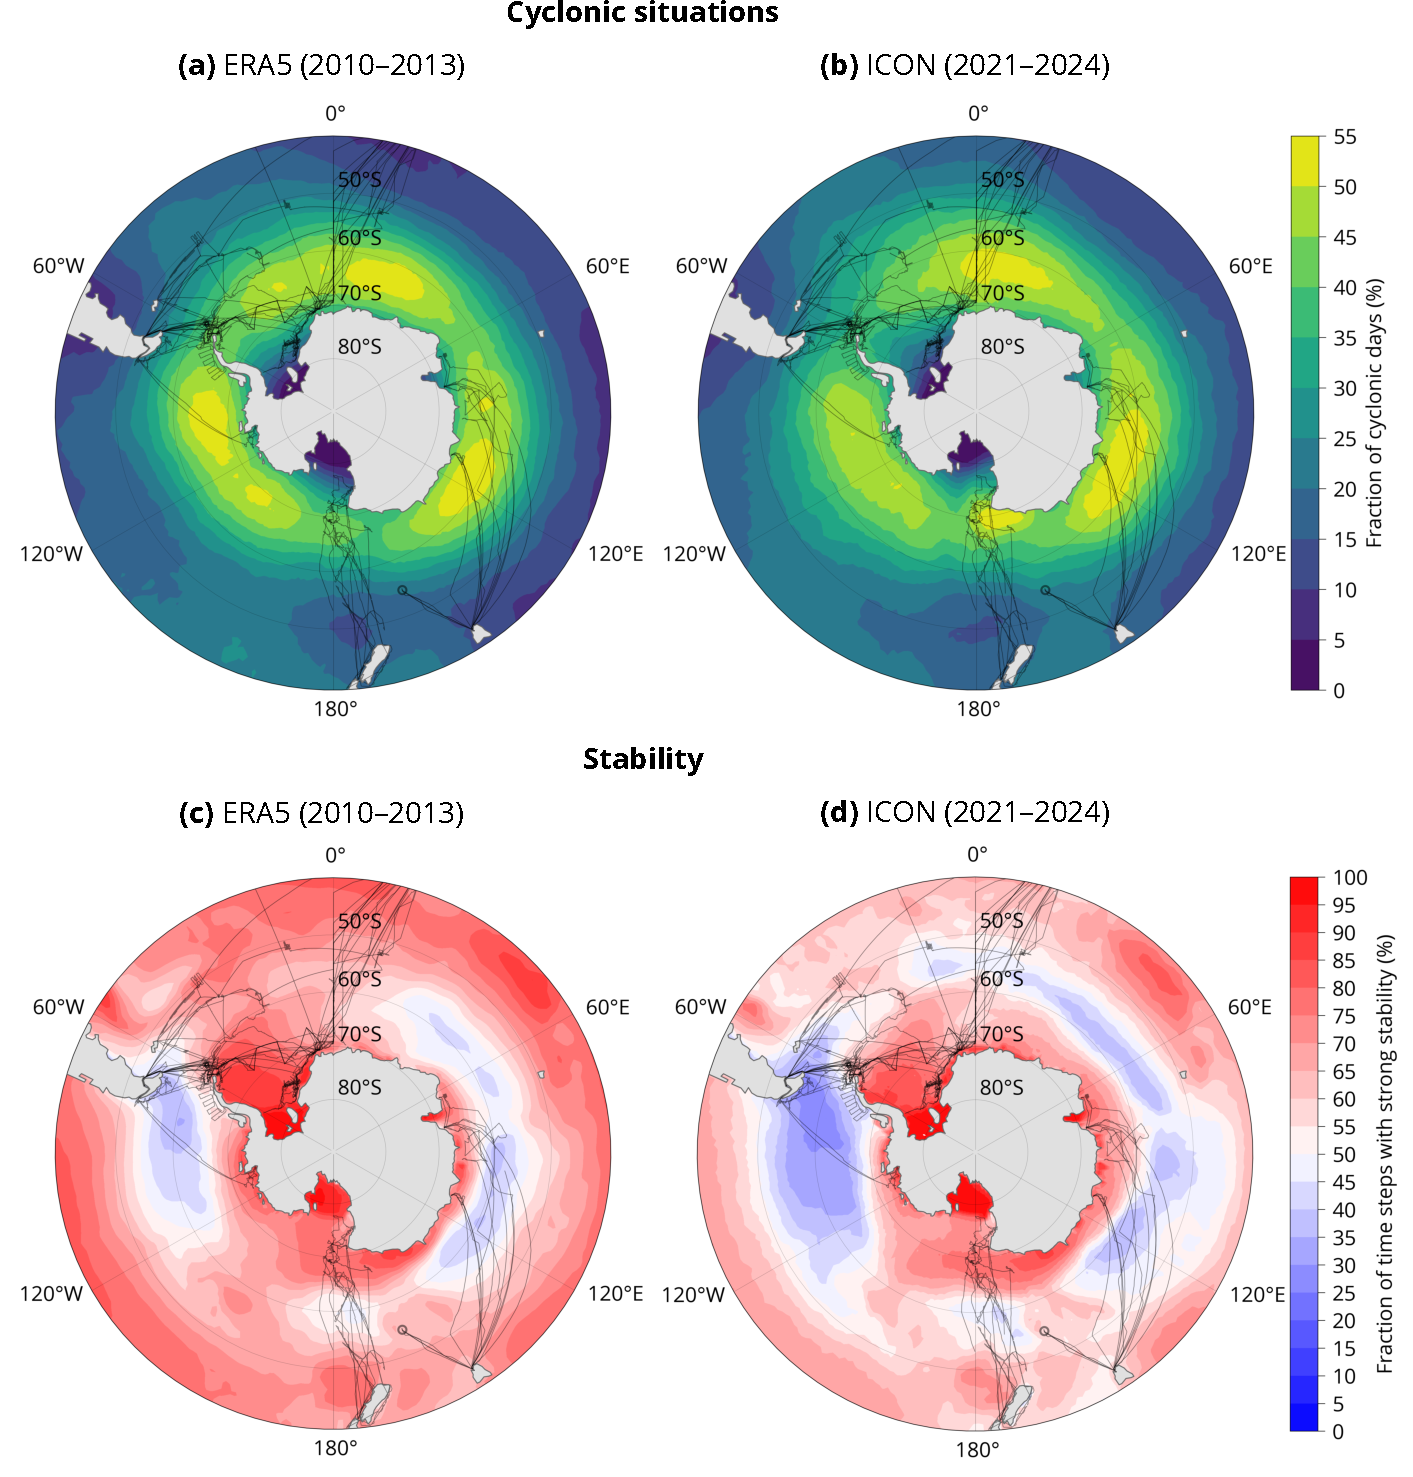
\includegraphics[width=\textwidth]{img/cyc_stab_dist_rev1.pdf}
\caption{
Geographical distribution of \textbf{(a, b)} cyclonic days and \textbf{(b, d)} strong stability (LTS~$\geq$~12~K) time steps in \textbf{(a, c)} ERA5 in years 2010--2013 (inclusive) and \textbf{(b, d)} ICON in model years 2021--2023 (free running). Cyclonic days are expressed as a fraction of the number of days with cyclonic activity, defined as grid points located within a double radius of any cyclone on a given day (UTC), as identified by CyTRACK. The voyage tracks and the point of the MICRE campaign are also shown.
}
\label{fig:cyclone-stability}
\end{figure}

\subsection{Cyclonic Activity and Stability}

Fig.~\ref{fig:cyclone-stability}a, b show the geographical distribution of the fraction of cyclonic days as determined by the cyclone tracking algorithm applied to the ERA5 reanalysis and ICON data (Section~\ref{sec:cyclone-stability}). As expected, the strongest cyclonic activity is in the high-latitude SO zone and is relatively zonally symmetric at all latitudes. The pattern matches reasonably well with \citeA{hoskins2005}. While both reanalysis and the model agree within about 8\% in most areas, ICON is prevailingly more cyclonic by about 4\%. There are clear differences, particularly in the highest occurrence rate regions, such as around Cape Adare, which is up to 20\% more cyclonic in ICON, and the Weddell and Bellingshausen Seas, where ICON is less cyclonic by up to 10\%. These differences might, however, stem from the relatively short time periods of comparison (4 years) and the fact that the model is free-running.

Fig.~\ref{fig:cyclone-stability}c, d show the geographical distribution of the conditions of weak and strong stability as determined by the LTS (Section~\ref{sec:cyclone-stability}). Conditions of weak stability are prevalent in the mid-to-high SO (50--65°S), which might be explained by the relatively cold near-surface air overlying the relatively warm sea surface. Conditions of strong stability are common elsewhere over the SO. The distribution is also less zonally symmetric than the cyclonic activity. In the high-latitude SO, the presence of sea ice might have a substantial stabilizing effect \cite{knight2024}. ICON is also substantially less stable than ERA5 across the whole region. In Section~\ref{sec:thermodynamic-profiles} we show that based on radiosonde observations, the bias is in ICON and not ERA5, and it is the result of underestimated temperature at heights corresponding to 700 hPa, as well as overestimated near-surface air temperature, characterized by a higher frequency of occurrence in the 1--7°C range compared to observations at radiosonde launch locations (Fig.~\ref{fig:stats-hist-surf}a). This may be related to large-scale circulation in the model or radiative transfer biases.

\subsection{Cloud Occurrence by Height}
\label{sec:cloud-occurrence}

We used the ALCF to derive cloud occurrence by height and the total cloud fraction from observations, ICON, ERA5, and MERRA-2. The results for all campaigns individually are shown in Fig.~\ref{fig:cloud-occurrence-panel}. As shown in this figure, the biases are relatively consistent across the campaigns and longitudes. In addition, we aggregated the campaigns by calculating the averages and percentiles of all individual profiles, presented in Fig.~\ref{fig:cloud-occurrence}. The analysis shows that the total cloud fraction is underestimated in ICON by about 10\% and in the reanalyses by about 20\%. When analyzed by height, ICON overestimates cloud occurrence below 1 km and underestimates it above; MERRA-2 underestimates cloud occurrence at all heights by up to 10\%, especially near the surface; and ERA5 simulates cloud occurrence relatively well above 1 km but strongly underestimates it near the surface. We note that fog or near-surface clouds are strongly underestimated in the reanalyses (fog and clouds are both included in the cloud occurrence). We conclude that the ICON results match the observations better than the reanalyses in this metric.

For all observations considered (Fig.~\ref{fig:cloud-occurrence}a), the data show cloud occurrence peaking near the surface, whereas the models show a higher peak (at about 500~m). The models generally underestimate the total cloud fraction by 10--30\% and show a strong drop in cloud occurrence near the surface, which is not identified in the observations. ICON and ERA5 overestimate cloud occurrence at their peak (between 0 and 1~km). Above 1~km, ICON and MERRA-2 underestimate cloud occurrence, but ERA5 is accurate to about 3\% or less. The exaggerated peak in models is partly explained by the lifting condensation level (LCL) distribution, which peaks about 300~m higher in the models than in the observations (near the surface), although this is not very pronounced. This is indicative of near-surface relative humidity often being close to saturation in the observations but not in the models (Fig.~\ref{fig:stats-hist-surf}b). There are multiple possible reasons for this bias, such as how the statistical distribution of RH within a grid cell is represented in the models, the air--sea moisture flux parameterization, or weaker stability in the models can cause more boundary mixing across heights and thus lower near-surface RH.

When subsetted by latitude (Fig.~\ref{fig:cloud-occurrence}b, c), we see that the low-latitude SO zone (40--55°S) displays a stronger peak of cloud occurrence near the surface than the high-latitude SO zone (between 55°S and the Antarctic coast), and this could be because higher latitudes have greater prevalence of weakly stable profiles (Fig.~\ref{fig:cyclone-stability}c, d), although more stable profiles populate regions south of 65°S close to the Antarctic coast. Cyclonic activity is also stronger in high-latitude SO, which is typically associated with shallow or deep convection rather than very stable stratification necessary for fog formation. The low- and high-latitude SO zones show similar biases in models as in the general case, but ERA5 does not overestimate the peak in the low-latitude SO zone (near-surface cloud occurrence is still strongly underestimated).

When subsetted by cyclonic and non-cyclonic situations (Fig.~\ref{fig:cloud-occurrence}d, e), we see that the cyclonic situations have a larger amount of observed cloudiness, including peak and total cloud fraction, by about 10\%. In the cyclonic situations, the model vertical profiles of cloud occurrence compare well with observations, but they peak higher by about 200 m and are larger by about 8\%. The reanalyses tend to underestimate cloud occurrence above 1 km by about 5\% and near the surface by about 15\%. Non-cyclonic situations are similar to the general case, also because they form the majority of analyzed profiles (83\%).

When subsetted by conditions of strong and weak stability (Fig.~\ref{fig:cloud-occurrence}f, g), as defined in Section~\ref{sec:cyclone-stability}, we see that in situations of strong stability, cloud occurrence peaks strongly near the surface in observations, compared to situations of weak stability, where the peak is more diffuse between 0 and 1~km. Physically, conditions of strong stability are associated with the formation of advection fog, such as in situations of warm air advection from the north over a colder sea surface, thus inducing fog formation by cooling of the warm and humid air by the cold surface. In situations of strong stability, the models have smaller biases than in weak stability, with an overestimated peak up to 12\%, underestimated cloud occurrence above 1~km by up to 5\%, and underestimated cloud occurrence near the surface by about 10\% in the reanalyses but not ICON. In situations of weak stability, the bias in ICON is very pronounced, with a much larger peak in cloud occurrence at about 500~m; the reanalyses underestimate cloud occurrence below 1~km, especially near the surface; and MERRA-2 underestimates cloud occurrence more strongly at almost all heights.

In all subsets, even when the models overestimate cloud occurrence at some altitudes, they always substantially underestimate the total cloud fraction. ICON can be generally characterized as substantially overestimating cloud occurrence below 1~km and underestimating above, underestimating the total cloud fraction, and showing the greatest biases in conditions of weak stability and non-cyclonic conditions. ICON also has a peak cloud occurrence at higher altitudes than observations (500~m vs. near the surface), and correspondingly, its LCL tends to be higher. MERRA-2 can be generally characterized as underestimating cloud occurrence at nearly all altitudes as well as the total cloud fraction, but mostly above and below 500~m (the peak at 500~m is well represented). MERRA-2 displays the largest errors relative to observations in the low-latitude SO zone and under weak stability. ERA5 can be generally characterized as representing cloud occurrence correctly above about 1.5~km, overestimating between 500~m and 1~km, but underestimating near-surface cloud occurrence (0--500~m). The total cloud fraction is strongly underestimated in all subsets. ERA5 has a tendency towards greater cloud underestimation in the low-latitude SO zone and under weak stability; conversely, it overestimates the peak of cloud occurrence at 500~m in the high-latitude SO zone and under strong stability.

\begin{figure}[p!]
\centering
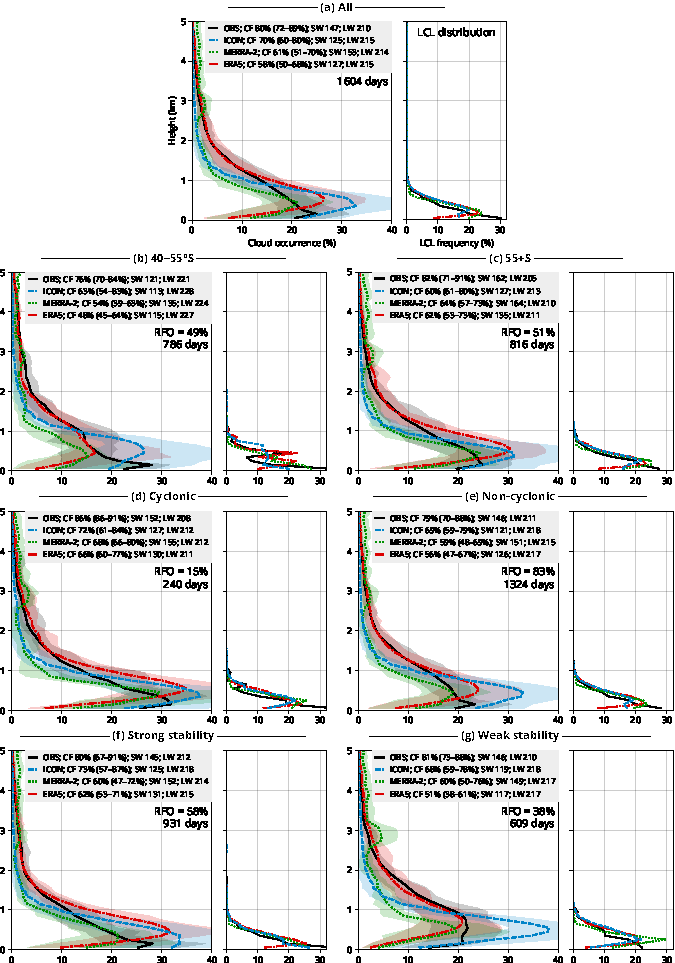
\includegraphics[width=\textwidth]{img/cl_agg_rev1.pdf}
\caption{
Cloud occurrence by height calculated as the average of all voyages and stations and lifting condensation level (LCL) distribution. The LCL is derived from radiosonde profiles and equivalent model profiles, which were not available for all voyages and times. The total cloud fraction (CF), average shortwave (SW), and longwave (LW) and the relative frequency of occurrence (RFO) are shown. The bands are the 16$^\mathrm{th}$--84$^\mathrm{th}$ percentile, calculated from the set of all voyages and stations.
}
\label{fig:cloud-occurrence}
\end{figure}

\subsection{Daily Cloud Cover}
\label{sec:cloud-cover}

We also analyzed the daily cloud cover (total cloud fraction) distribution. This is a measure of cloudiness, irrespective of height, calculated over the course of a day (UTC). A cloud detected at any height means that the lidar profile was classified as cloudy; otherwise, it was classified as a clear sky. When all profiles in a day are taken together, the cloud cover for the day is defined as the fraction of cloudy profiles in the total number of profiles, expressed in oktas (multiples of 1/8). The same calculation is done for the lidar observations as for the simulated lidar profiles. We use the term ``okta'' independently of its use in instantaneous synoptic observations, and here it simply means 1/8 (0.125) of the daily cloud cover.

In Fig.~\ref{fig:cloud-cover} we show the results for the same subsets of data as in Section~\ref{sec:cloud-occurrence}. Observations display the highest proportion of high cloud cover values (5--8~oktas), peaking at 7~oktas. This pattern is not represented by ICON or either reanalysis. While ICON is closest to matching the observed distribution, it tends to be 1~okta clearer than the observations, peaking at 6~oktas, and substantially underestimating days with 8~oktas. Overall, the reanalyses show results similar to each other, underestimating cloud cover by about 2~oktas and strongly underestimating days with 7 and 8~oktas. Of the two reanalyses, MERRA-2 has slightly higher cloud cover than ERA5, by about 6\% at 6 octas, which makes it more consistent with observations.

When analyzed by subsets, observations in the cyclonic subset show the highest cloud cover, with 8~oktas occurring on one half of such days (Fig.~\ref{fig:cloud-cover}d). This sensitivity to cyclonic conditions is not observed in ICON or the reanalyses. Interestingly, clear sky days (0~oktas) also have a local maximum peaking at about 15\% in this subset. When we contrast the low- and high-latitude zones, we see that the high-latitude zone tends to have greater cloud cover, peaking at 8~oktas (Fig.~\ref{fig:cloud-cover}c). The high-latitude zone also has almost no clear sky or small cloud cover cases (0--4~oktas). ICON and the reanalyses represent this characteristic of the distribution well for 0--3~oktas, but otherwise show biases similar to the general case. One of the greatest biases is present in ERA5 in the subset of weak stability, in which ERA5 peaks at 3~oktas, while the observations peak at 7~oktas and show negligible cloud cover below 5~oktas.

\begin{figure}[p!]
\centering
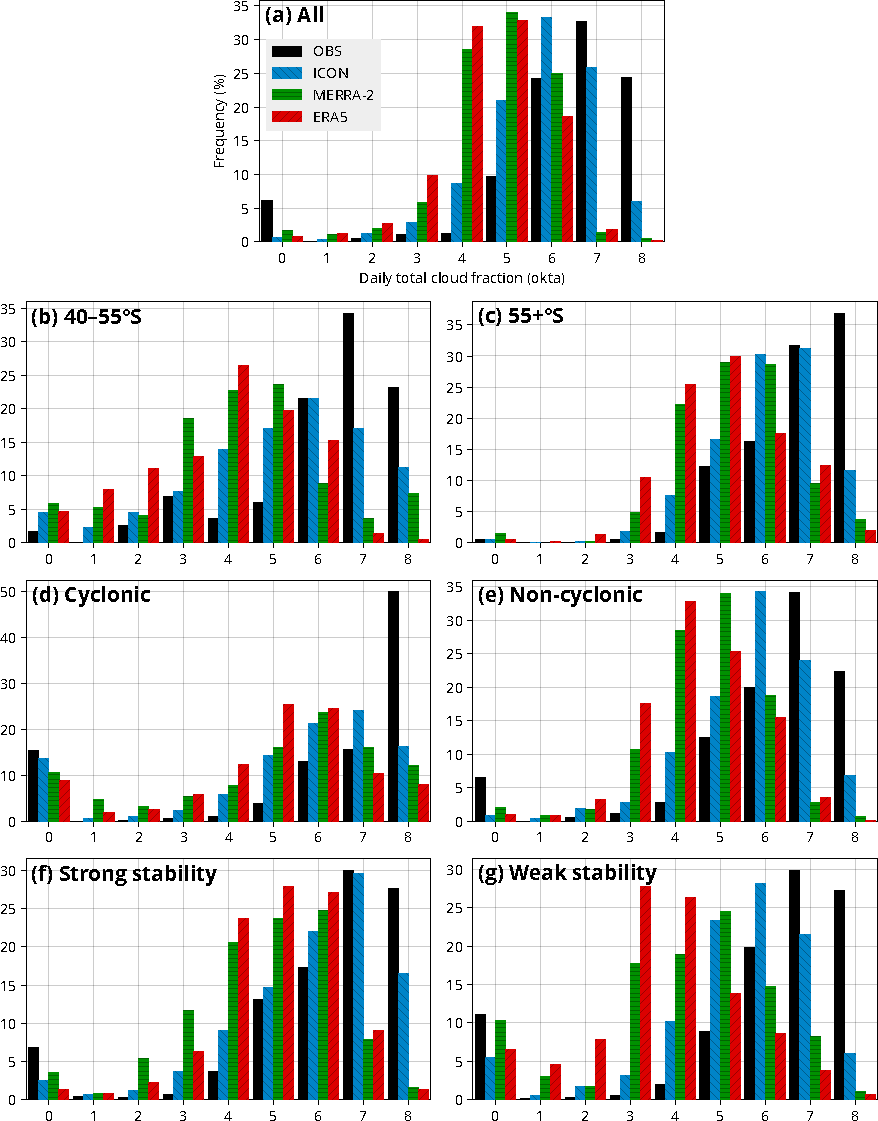
\includegraphics[width=\textwidth]{img/clt_hist_rev1.pdf}
\caption{
Daily total cloud fraction histograms calculated as the average of all voyage and station histograms. The total cloud fraction of a day (UTC) is calculated as a fraction of cloudy (based on the cloud mask) observed (OBS) or simulated lidar profiles. The models and subsets are as in Fig.~\ref{fig:cloud-occurrence}.
}
\label{fig:cloud-cover}
\end{figure}

\subsection{Top of Atmosphere Radiation, Liquid and Ice Water Path}

In Fig.~\ref{fig:cloud-occurrence}, we also show the mean outgoing shortwave and longwave top-of-atmosphere radiation, whose calculation is described in Section~\ref{sec:ceres}. In observations, these come from daily mean CERES measurements averaged over the voyage tracks or a station location, whereas in the models they come from daily means of TOA radiation in the model output averaged over the same location and time periods.

In the general case (Fig.~\ref{fig:cloud-occurrence}a), ICON and ERA5 underestimate the outgoing SW radiation by 22 and 20 Wm$^{-2}$ (respectively), and MERRA-2 overestimates it by 6 Wm$^{-2}$. While in ICON and ERA5, this is in line with the underestimated total cloud fraction of 10\% and 22\% (respectively); in MERRA-2, the opposite result is expected from the underestimated total cloud fraction of about 20\%. Neglecting the direct radiative effects of sea and aerosol, this is only possible if the albedo of cloudy areas is overestimated, compensating for the lack of cloudy areas.

We note that the radiative transfer calculations used in the lidar simulator mean that the impact of both cloud phase and cloud fraction are convolved to produce the cloud mask. Therefore, the cloud occurrence is not affected by any cloud phase biases as long as the cloud is optically thick enough to be detected and the laser signal is not too attenuated. A combination of underestimated total cloud fraction and overestimated outgoing SW at TOA is indicative of an overestimated cloud albedo (in cloudy areas) due to either cloud liquid and ice water content, cloud phase, droplet or ice crystal size distribution, shape or orientation of ice crystals, cloud overlap, or their combination. The influence of cold clouds is likely second-order due to the much larger typical effective radius of ice crystals than cloud droplets.

In contrast to SW radiation, the models have much smaller LW radiation biases, which is expected due to the prevailing low-level clouds having similar temperatures as the surface. \citeA{roh2021} also found LW biases to be much lower than SW biases in DYAMOND models over the tropical Atlantic Ocean. In ICON, the outgoing LW radiation is overestimated by 5\% (Fig.~\ref{fig:cloud-occurrence}a). This is likely caused by an underestimated total cloud fraction exposing a larger sea surface area to cooling to space, which is typically warmer than the atmospheric temperature at 0--2~km, where most of the clouds are located. In the MERRA-2 and ERA5 reanalyses, the LW biases are also slightly positive, 4 and 5~Wm$^{-2}$, respectively. This is again in line with the underestimated total cloud fraction by about 20\%. However, if the clouds are too thick, as expected from the SW results, this might also provide a compensating effect, in which too small a cloud area is counteracted by greater optical thickness in the LW spectrum, thus reducing the outgoing LW radiation more relative to thinner clouds. For thin clouds, the outgoing TOA LW radiation originates both from the warmer surface (partly blocked by the clouds) and the clouds, whereas for thick clouds, the outgoing TOA LW radiation originates mostly from the colder-than-surface clouds.

In all the subsets (Fig.~\ref{fig:cloud-occurrence}b--g), the same type of biases are observed, namely the outgoing SW radiation is underestimated in ICON and ERA5 and overestimated in MERRA-2, and the outgoing LW radiation is overestimated in all the models. Even though the total cloud fraction is higher by 6\% over the high-latitude SO than the low-latitude SO, the outgoing SW radiation is much greater by 41~Wm$^{-2}$, implying a much greater cloud albedo (of cloudy areas) over the high-latitude SO. ICON has little difference in the total cloud fraction between low- and high-latitude SO, but greater outgoing SW radiation by 14~Wm$^{-2}$ over the high-latitude SO, likely due to thicker clouds under deeper convection in less stable and more cyclonic conditions relative to the low-latitude SO. In contrast, the reanalyses showed both greater total cloud fraction and outgoing SW radiation over the high-latitude SO compared to the low-latitude SO.

Fig.~\ref{fig:stats-hist} shows the SW and LW radiation, liquid water path (LWP), and ice water path (IWP) distributions as histograms and their corresponding averages. LWP and IWP are calculated from the mass of water in the column divided by the area of the column, i.e. not just the area of the cloudy portion of the column, as in some definitions. ERA5 and ICON overestimate outgoing SW near 80 Wm$^{-2}$ (Fig.~\ref{fig:stats-hist}a), which probably relates to clear sky situations, as expected from the underestimated cloud fraction. They also underestimate the highly reflective situations above 200 Wm$^{-2}$. MERRA-2 exhibits the too few, too bright problem in terms of overestimating SW reflectivity around 290 Wm$^{-2}$, given that the total cloud fraction in MERRA-2 is strongly underestimated. The LW distribution shows that all of the models overestimate outgoing LW (Fig.~\ref{fig:stats-hist}b), which is expected from the underestimated cloud fraction, exposing more of the warmer ocean surface relative to colder clouds. The LWP distribution shows that all models overestimate cases with near-zero LWP (Fig.~\ref{fig:stats-hist}c), which relates to the underestimated total cloud fraction. MERRA-2 shows quite overestimated high-LWP situations, which is most likely related to the too few, too bright problem of simulating lower total cloud fraction but clouds with higher LWP to compensate. IWP (Fig.~\ref{fig:stats-hist}d) is somewhat less important radiatively than LWP because of the typically larger and less numerous hydrometeors. Similarly to LWP, the models overestimate situations with near-zero IWP. ERA5 is otherwise simulating the IWP distribution well, but ICON and MERRA-2 underestimate IWP. Fig.~\ref{fig:stats-hist-cloudy} shows the same as Fig.~\ref{fig:stats-hist}, but for cloudy profiles only. This figure shows more distinctly that in cloudy situations, MERRA-2 overestimates moderate (0.05--0.15 kg m$^{-2}$) and high LWP (over 0.15 kg m$^{-2}$), and ERA5 and ICON underestimate moderate LWP. ICON also overestimates high LWP, resulting in overestimated average LWP.

\begin{figure}[t]
\centering
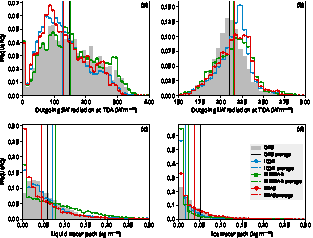
\includegraphics[width=\textwidth]{img/stats_hist.pdf}
\caption{
Histograms and averages of outgoing \textbf{(a)} SW and \textbf{(b)} LW radiation at TOA, \textbf{(c)} liquid water path, and \textbf{(d)} ice water path in CERES SYN1deg observations (OBS), ICON, MERRA-2, and ERA5 along the voyage tracks. All voyages are weighted equally. The statistics are calculated from daily mean values corresponding to each time step and geographical location of the voyage tracks.
}
\label{fig:stats-hist}
\end{figure}

\begin{figure}[p!]
\centering
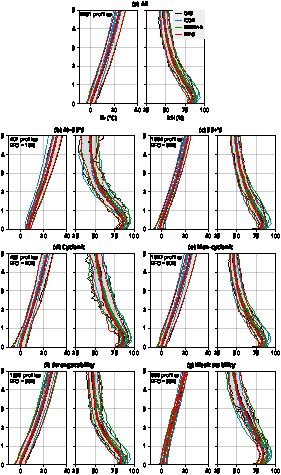
\includegraphics[width=0.85\textwidth]{img/rs_agg_rev1.pdf}
\caption{
Virtual potential temperature (virt.\ pot.\ temp.; $\theta_v$) and relative humidity (RH) determined from radiosonde launches and co-located profiles in ICON, ERA5, and MERRA-2 in subsets as in Fig.~\ref{fig:cloud-occurrence}. The solid lines are the average calculated from the averages of every individual voyage and station. The bands span the 16$^\mathrm{th}$--84$^\mathrm{th}$ percentiles, calculated from the distribution of the voyage and station averages. Shown is also the relative frequency of occurrence and the number of profiles in each subset.
}
\label{fig:potential-temperature}
\end{figure}

\subsection{Relative humidity and potential temperature profiles}
\label{sec:thermodynamic-profiles}

In order to examine the potential link in the cloud biases to the local physical conditions, we analyzed about 2300 radiosonde profiles south of 40°S available from the 24 RV \emph{Polarstern} voyages and the MARCUS, NBP1704, TAN1702, and TAN1802 campaigns. Spatially and temporally colocated profiles were taken from ICON and the reanalyses. Because the time period covered by the ICON model output (2021--2024) was different from the time period covered by the observations (2010--2021), when comparing with the model, we first had to remap the observation time to model time by taking the same time relative to the start of the year. Consequently, we also had four virtual/model profiles (one for each year from 2021 to 2024) for each observed profile. The profiles were partitioned into the same subsets as above (Sections~\ref{sec:cloud-occurrence} and \ref{sec:cloud-cover}). We focus on comparing virtual potential temperature ($\theta_v$) and relative humidity, being one of the primary factors affecting shallow convection and the associated low-level cloud formation and dissipation. The observed and model profiles of virtual potential temperature and relative humidity are shown in Fig.~\ref{fig:potential-temperature}.

Overall, the mean $\theta_v$ is accurate to within 0.5~K in ICON and MERRA-2, except for ICON being colder by up to 2.5~K in the mid-to-high troposphere (less stable) (Fig.~\ref{fig:potential-temperature}a). Larger differences exist, however, in the 40--55°S zone, where ICON is colder by about 5 K at higher altitudes (Fig.~\ref{fig:potential-temperature}b). In other subsets, the bias is relatively small. MERRA-2 and ERA5 are very close to the observations, possibly due to a high accuracy of assimilation of this quantity. Notably, the variability of virtual potential temperature (as represented by the percentiles) is much smaller in ICON than in the observations. This indicates that the model's internal variability in the lower-tropospheric thermodynamic conditions in the SO is smaller than in reality.

Relative humidity displays much larger biases. In all subsets, ICON is too humid in the first 1~km by about 5\%, but very accurate above, except for the 40--55°S zone and conditions of weak stability (Fig.~\ref{fig:potential-temperature}b, g), where it is too dry between about 1 and 3~km. Even though relative humidity measured by radiosondes in the first 100~m is not very different between the observations and the models (Fig.~\ref{fig:potential-temperature}a), near-surface (2-m) relative humidity at the radiosonde launch locations is much greater in the observations, most often close to 100\%, unlike in the models, where 85\% tends to be the most common (Fig.~\ref{fig:stats-hist-surf}b). This also explains why LCL is much more frequently located at the surface in the observations than in the models (Fig.~\ref{fig:cloud-occurrence}a). LCL is fully determined by near-surface temperature, near-surface relative humidity, and surface pressure.

\begin{figure}[t]
\centering
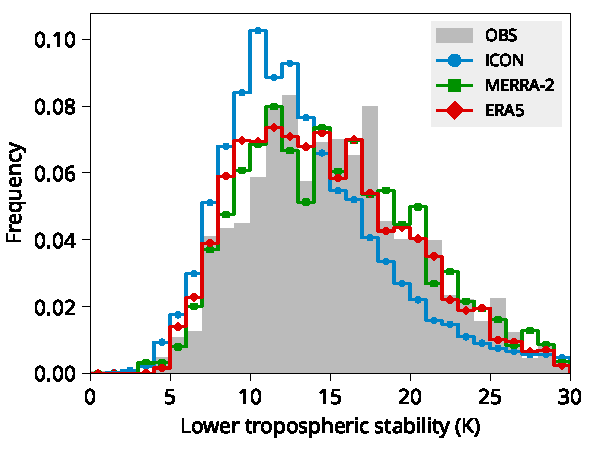
\includegraphics[width=0.6\textwidth]{img/rs_lts_hist.pdf}
\caption{
Histogram of lower tropospheric stability calculated from the observed radiosonde profiles and the corresponding model profiles. All campaigns are weighted equally.
}
\label{fig:rs-lts-hist}
\end{figure}

\begin{figure}[t]
\centering
\makebox[\textwidth][c]{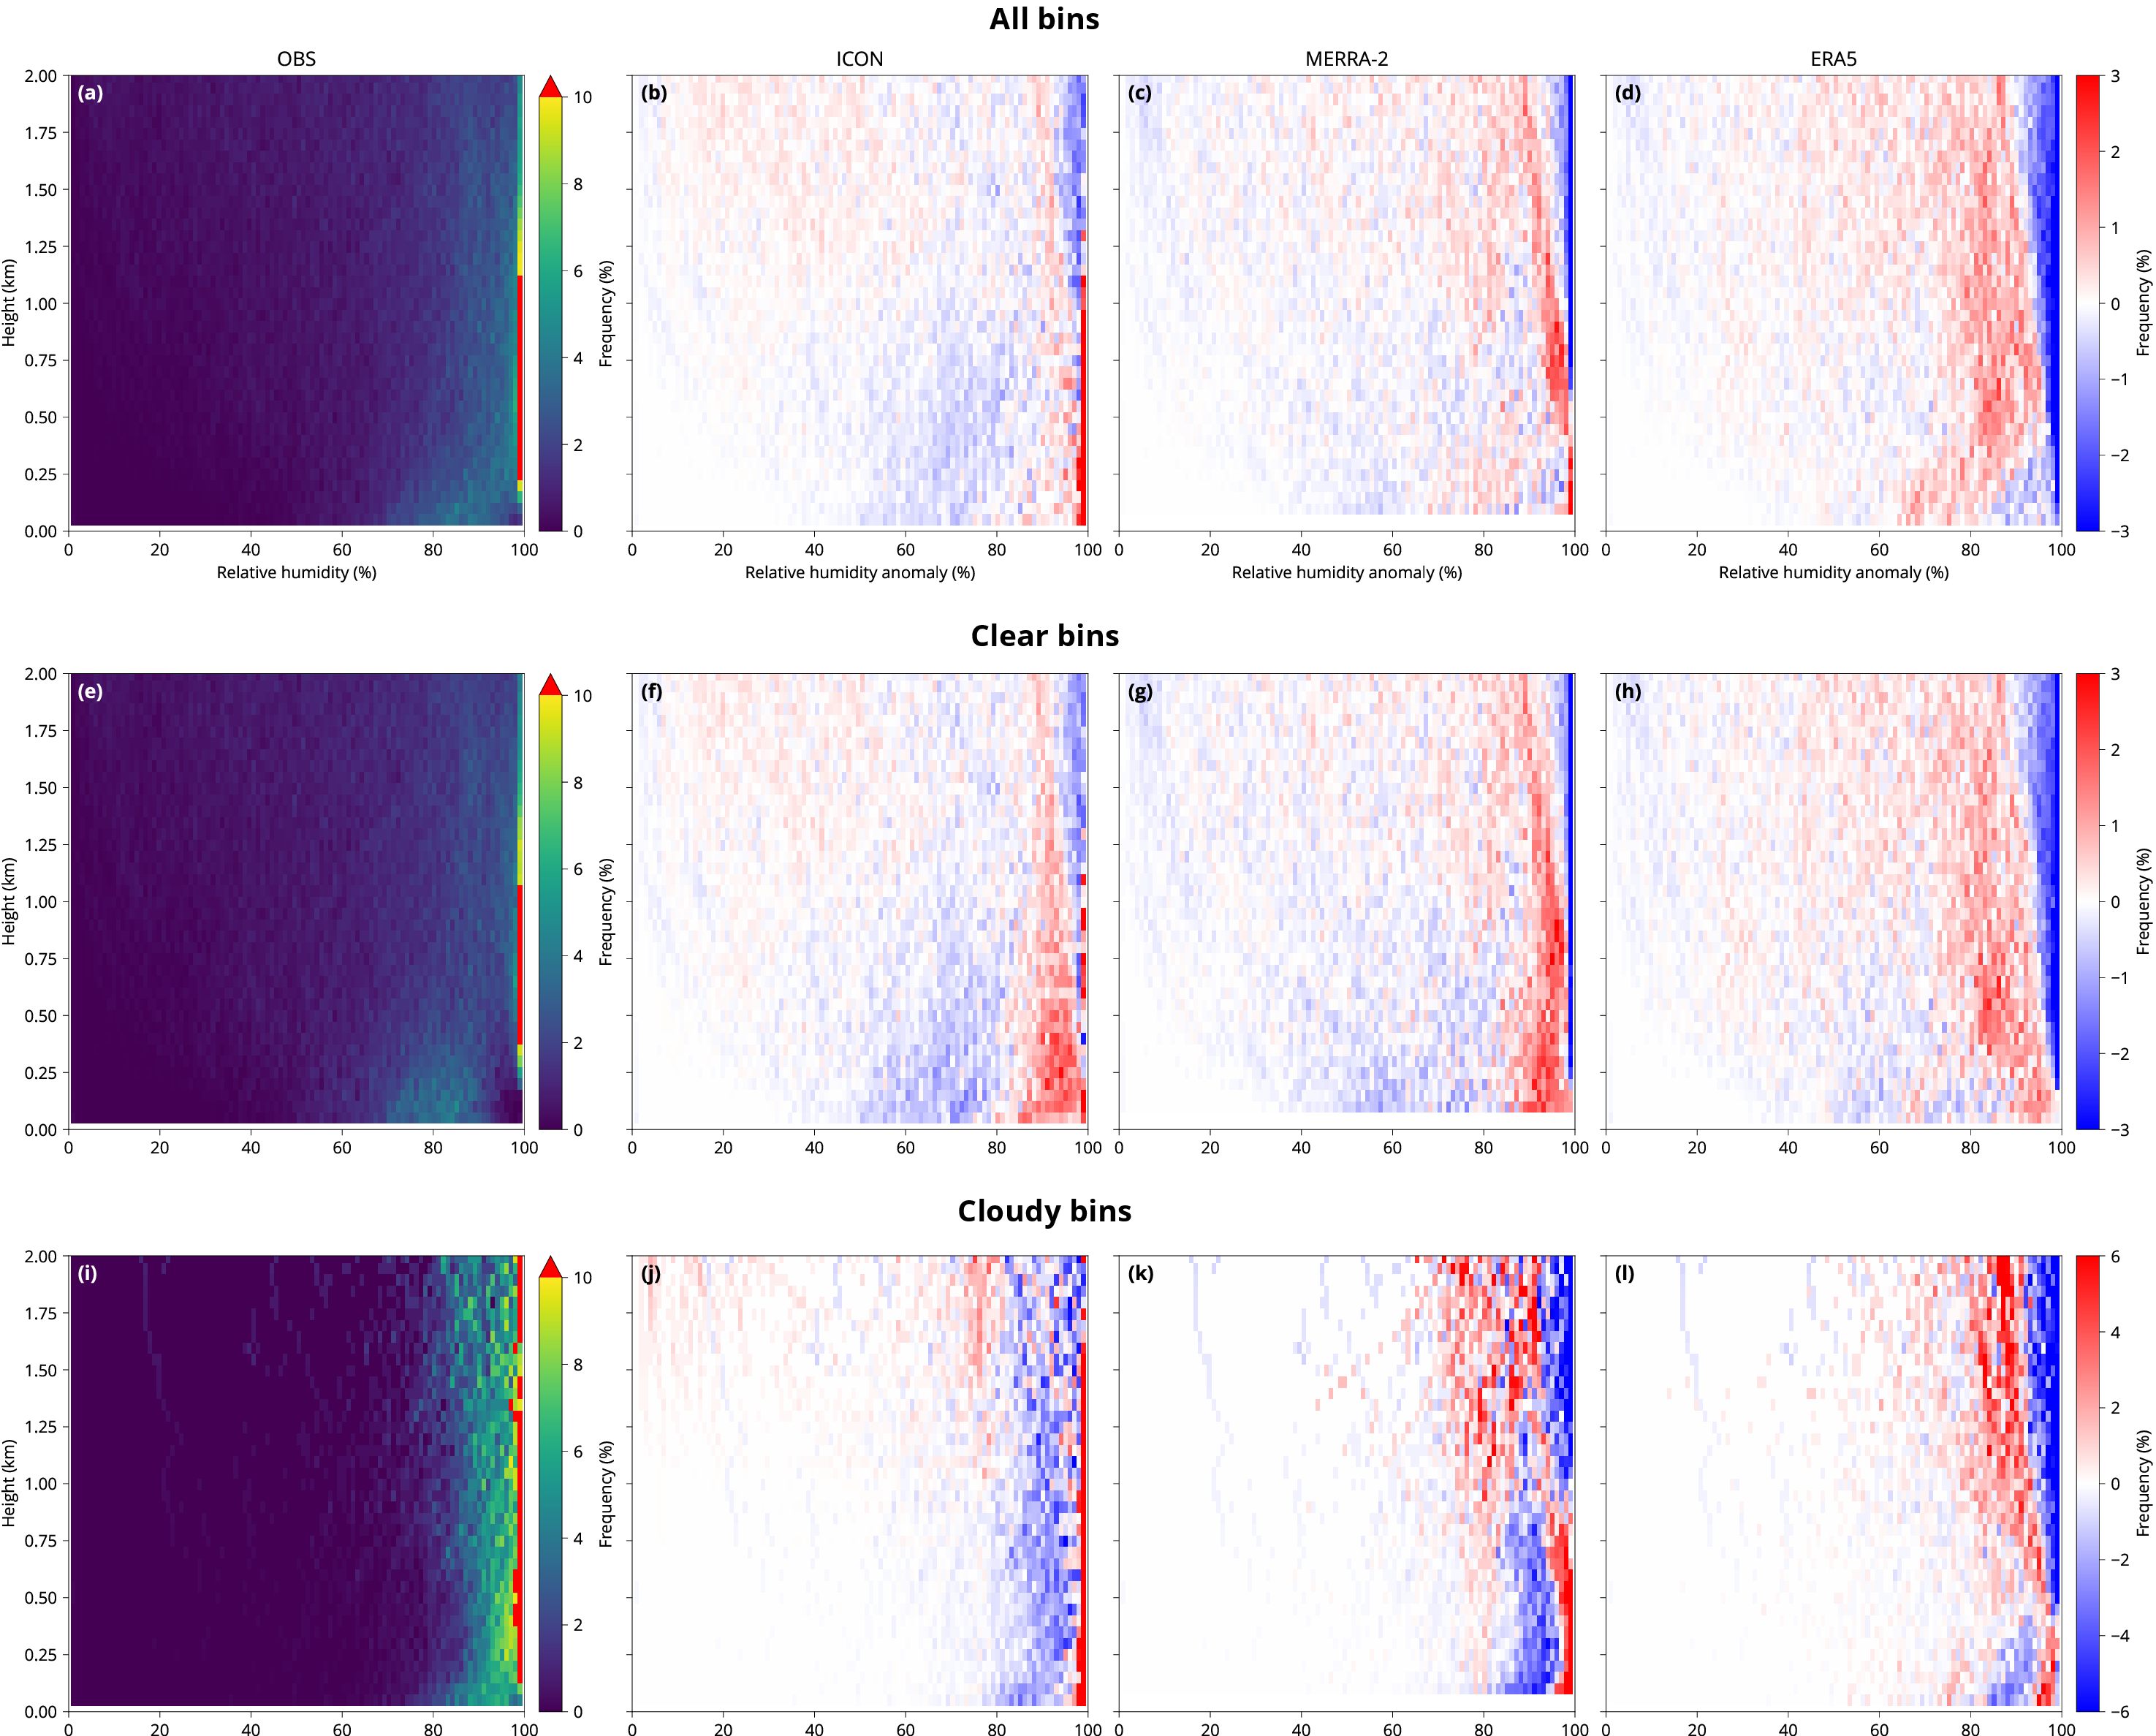
\includegraphics[width=1.3\textwidth]{img/rs_hur_hist.png}}
\caption{
Relative humidity histograms calculated from the observed radiosonde profiles and the equivalent model profiles for \textbf{(a)} all bins, \textbf{(b)} clear bins, and \textbf{(c)} cloudy bins, determined from the lidar cloud mask. Model histogram values are relative to observations. The histogram values are normalized to 100\% for each level separately. All campaigns are weighted equally.
}
\label{fig:rs-hur-hist}
\end{figure}

Fig.~\ref{fig:rs-thetav-hur-cloud} shows virtual potential temperature and RH profiles for profiles containing fog, cloud at 500 m, and cloud at 1.5 km. These situations are characterized by particular cloud biases as identified in the lidar cloud occurrence analysis. The rationale is to examine $\theta_v$ and RH associated with these situations. Foggy situations are characterized by a rapid increase of $\theta_v$ with height and an observed average RH of about 90\% near the surface (Fig.~\ref{fig:rs-thetav-hur-cloud}a). In contrast, the models simulate higher RH in the first 100~m under foggy conditions by several percentage points. In situations with clouds occurring at 500 m, $\theta_v$ is relatively flat between the surface and 500 m (Fig.~\ref{fig:rs-thetav-hur-cloud}b), as expected for convectively driven clouds. The observed RH peaks at 500 m at about 90\%. The models, however, simulated higher RH between the surface and 500 m under these conditions. ICON and ERA5 show a stronger decrease of RH above this height than observations, and ERA5 shows more strongly stable stratification. Unlike the foggy and 500-m cloud situations, situations with clouds at 1.5 km do not have a flat $\theta_v$ with height. This indicates that unlike the former, clouds at 1.5 km are not (or not as strongly) convectively driven. As expected, RH in these situations peaks at 1.5 km at about 85\% in observations. In the models, this peak is much less pronounced.

Fig.~\ref{fig:rs-lts-hist} shows the histogram of LTS calculated from all radiosonde profiles and the corresponding profiles in the models. It can be seen that ICON substantially underestimates the occurrence of cases of strong stability above 16 K while overestimating the cases of moderate stability (8 to 16 K). When considered together with the cloud occurrence results presented in Fig.~\ref{fig:cloud-occurrence}, we see that since the model is biased towards weak stability, it overrepresents cloud profiles strongly peaking at 500 m (Fig.~\ref{fig:cloud-occurrence}g) over cloud profiles with fog or near-surface cloud (Fig.~\ref{fig:cloud-occurrence}f). This can be a physical reason for its overall positive bias in cloud at 500 m (Fig.~\ref{fig:cloud-occurrence}a) instead of the observed cloud occurrence profile peaking near the surface. The reanalyses simulate the LTS distribution well except for a slight underestimation of LTS.

Fig.~\ref{fig:rs-hur-hist} shows RH histograms calculated from the radiosonde observations and equivalent profiles in the models (shown as anomalies relative to the observations), calculated for all, clear, and cloudy bins, based on the lidar observations and the simulated lidar backscatter in the models. Here, we show only the first 2 km to concentrate on the identified cloud biases seen at these heights. We can see several notable features. The models simulate progressively fewer high-RH (\textgreater 90\%) bins above the ground (Fig.~\ref{fig:rs-hur-hist}b--d). This can be related to either ice nucleation happening in the models, which requires smaller RH for saturation, or the grid cell size in the models, which requires lower grid cell average RH than 100\% for saturation to occur in a fraction of the grid cell. The models also tend to simulate more clear bins than observations for RH between 80 and 100\% between the ground and about 1 km (Fig.~\ref{fig:rs-hur-hist}f--h). In observations, these values of RH are associated with cloudy bins (Fig.~\ref{fig:rs-hur-hist}i). Conversely, the models predominantly associate only RH very close to 100\% with cloudy bins at these heights (Fig.~\ref{fig:rs-hur-hist}j--l). This may be one of the main reasons for the identified cloud or fog biases near the ground. A possible explanation is that cloud droplets are able to form or persist at RH between 90 and 100\% at these heights over the SO. This could be due to abundant sea salt or biogenic aerosol or droplet generation from sea spray in the common high swell and high wind speed conditions over the SO. Stratus fractus or other broken clouds could also lead to less than 100\% RH when averaged over the size of the vertical bins (up to 30 m in some of the radiosonde profiles).

Fig.~\ref{fig:rs-thetav-hist} shows histograms the same as the previous figure, but for virtual potential temperature. They show a more complex picture, characterized by a central peak at about 0°C near the surface, increasing to about 5°C at 2 km (Fig.~\ref{fig:rs-thetav-hist}a). For cloudy bins, the central peak is generally flatter with height and even shows a minimum in $\theta_v$ at about 500 m (Fig.~\ref{fig:rs-thetav-hist}i). This is indicative of convection being associated with clouds at these heights, which results in flat virtual potential temperature profiles. In the reanalyses, in the first 200 m, values slightly above 0°C are associated with more clear bins than in observations, and values slightly below 0°C with fewer (Fig.~\ref{fig:rs-thetav-hist}g--h). Conversely, the opposite is true for cloudy bins (Fig.~\ref{fig:rs-thetav-hist}k--l). Situations with 0°C near-surface air temperature might occur predominantly when open ocean surface keeps the near-surface air temperature close to 0°C under otherwise colder air mass conditions, such as under cold advection. ICON displays a notable bias above about 1 km, where the central peak is strongly underestimated (Fig.~\ref{fig:rs-thetav-hist}j). Instead, these heights and values of $\theta_v$ are more associated with clear bins (Fig.~\ref{fig:rs-thetav-hist}f). This might be related to the strong underestimation of cloud occurrence at these heights.

\section{Limitations of this Study}
\label{sec:limitations}

Let us consider the main limitations of the presented results. The spatial coverage of our dataset does not include most parts of the Indian Ocean and Pacific Ocean sectors of the SO. Even though climatological features of the SO are typically relatively uniform zonally, variations exist, such as those related to the Antarctic Peninsula and the southern tip of South America. The voyages were mostly undertaken in the Austral summer months and only rarely in the winter months, due to the poor accessibility of this region during winter. Therefore, our results are likely representative of summer and, to a lesser extent, spring and autumn conditions. Cloud regimes and phase in the region are seasonally variable \cite{danker2022}.

The time period of ICON is relatively short, with only four full years of simulation available. Moreover, the simulation is free-running and ocean-coupled, which means that observations had to be temporally mapped to this time period (at the same time relative to the start of the year) for the comparison. For these reasons, one can expect the results to be slightly different due to reasons unrelated to model biases, such as different weather conditions, partially accounted for by the cyclone and stability subsetting, and the phase of climate oscillations such as the ENSO in the observations and the model. The interannual variability in cloud occurrence in ICON can be seen in Fig.~\ref{fig:cloud-occurrence-panel}, where each year in ICON is represented by a separate line. As could be expected, the interannual variability tends to be substantially smaller than the biases and thus is unlikely to have a strong impact on the main findings.

It would be possible to use short-term ICON simulations for almost one-to-one comparison to observations. However, here we focus on long-term biases, which are statistically more robust. Our analysis is, therefore, complementary to shorter process-level studies. The reanalyses pose the difficulty of determining how much assimilated observations impact the results. While one might expect temperature and RH profiles to be well represented in the reanalyses due to assimilation of satellite data, we see that this is not always the case in comparison with the radiosonde profiles and near-surface meteorological observations. This could be due to the limited vertical accuracy of satellite sounding measurements and obscuration by clouds. Despite the assimilation, the cloud and radiation biases are often comparable to or greater than in the free-running model.

Ground-based lidar observations are affected by attenuation by thick cloud layers, and for this reason the results are most representative of boundary layer clouds, while higher-level clouds are only occasionally visible to the lidar when boundary layer clouds are not present. Ground-based lidar observations can be regarded as complementary to satellite lidar observations for the evaluation of low-level clouds, which are predominant in this region, while mid- and high-level clouds are likely better sampled by satellite observations \cite{mcerlich2021}. Ground-based observations are, however, complicated by precipitation, and satellite observations can also be used if the effect of overlapping clouds is carefully eliminated. Near-surface lidar retrievals ($\sim$100~m) are affected by uncertainties related to incomplete overlap, signal saturation (dead time), and after-pulse effect corrections \cite{kuma2021}.

Supercooled liquid clouds (liquid clouds under subzero temperature) commonly occur over the SO. In our analysis of LWP and IWP, we see that both phases are abundant. Because liquid water droplets are typically smaller and more numerous than ice crystals in cold clouds, they attenuate a greater amount of the lidar radiation. Clouds with a relatively modest optical thickness of 1.7 can attenuate the lidar signal for a detection at 2 km using an instrument with noise properties like the Vaisala CL31 (Section 2.4). While supercooled liquid clouds and their attenuation are accounted for by the lidar simulator, they can strongly attenuate the signal and cause artifically low values of cloud occurrence at higher altitudes. For example, we found that cloud occurrence at 1.5 km is underestimated in ICON and underlying clouds are overestimated. However, this can also mean that clouds at 1.5 km are present in the model but the signal is too attenuated by the lower clouds in the model but not in the observations, where the underlying clouds are not as pronounced.

We have attempted to remove lidar profiles with precipitation (about 26\% of all profiles), which could not be properly simulated with the lidar simulator (Section~\ref{sec:ann}). However, the approach was limited by the relatively low sensitivity of the ANN (65\%) and the fact that we had to choose a fixed threshold for surface precipitation flux in the model and reanalyses, which might not correspond to detection by the ANN applied to observations. We also made no attempt to remove profiles with precipitation that did not reach the surface. The above reasons may result in an artificial bias in the comparison, though we expect this to be much smaller than the identified model biases.

Subsetting by cyclonic activity and stability is done based on the ERA5 data. As we have shown, the reanalyses also suffer from biases in near-surface and upper-level quantities. Therefore, the subsetting is limited by the accuracy of the ERA5 pressure field, near-surface temperature, and temperature at 700~hPa. Near-surface ship observations are affected by the ship structures as well as the variable height above sea level at which the measurements are taken. The accuracy of radiosonde measurements in the first tens of meters from the surface is also likely affected by the ship environment, such as turbulence generated by ship structures and the ship exhaust. Vertical averaging of the radiosonde data can result in lower RH near saturation due to averaging of drier and moister layers together. For example, some of the RV \textit{Polarstern} radiosondes are available in vertical resolution of about 20--30 m. The satellite retrieval of LWP is affected by large biases, especially over high latitudes \cite{khanal2020}, which limits our comparison with the models.

\section{Discussion and Conclusions}

\begin{table}[t]
\caption{Summary of the main biases. Values are relative to observations and rounded to the nearest 5, except for daily cloud cover and RH, which are rounded to the nearest integer. The best-performing value is marked in \textbf{bold}. Abbreviations: boundary layer (BL), relative humidity (RH), shortwave (SW), longwave (LW), liquid water path (LWP), ice water path (IWP), and lifting condensation level (LCL).}
\label{tab:summary}
\centering
\begin{tabular}{llll}
& ICON & MERRA-2 & ERA5\\
\hline
Total cloud fraction (\%) & \textbf{-10} & -20 & -20\\
Daily cloud cover (okta) & \textbf{-1} & -2 & -2\\
Fog (\%) & \textbf{0} & -10 & -10\\
BL clouds (at $\sim$500 m) & 15 & \textbf{0} & 5\\
Mid-lev. clouds (at $\sim$1.5 km) & -5 & -5 & \textbf{0}\\
RH at 500 m & 2 & 2 & \textbf{0}\\
SW (W m$^{-2}$) & -25 & \textbf{5} & -20\\
LW (W m$^{-2}$) & 5 & 5 & 5\\
LWP (g m$^{-2}$) & \textbf{10} & 20 & -15\\
IWP (g m$^{-2}$) & -30 & -30 & \textbf{-15}\\
LCL distribution peak (m) & 300 & 300 & 300\\
\hline
\end{tabular}
\end{table}

We analyzed a total of about 2400 days of lidar and 2300 radiosonde observations from 31 campaigns and the Macquarie Island subantarctic station, covering the Atlantic, Australian, and New Zealand sectors of the SO over 10 years. This dataset, together with the use of a ground-based lidar simulator, provided a comprehensive basis for evaluating SO cloud and thermodynamic profile biases in the GSRM ICON and the ERA5 and MERRA-2 reanalyses. Our analysis provides a unique evaluation perspective, complementary to satellite observations for evaluating boundary layer clouds and fog, which are predominant in this region. We did not, however, analyze the cloud phase based on ground-based observations. Cloud phase can have a strong impact on the SW radiative transfer due to larger and therefore less numerous hydrometeors (for the same amount of water) scatter much less SW radiation. Especially underestimation of fog or near-surface clouds is very strong in the reanalyses, and we showed that this relates to cloud formation or persistence at RH between 80 and 100\% in the boundary layer in the observations, while in models RH values less than 100\% are associated with clear bins. We subsetted the dataset by low and high latitude SO bands, cyclonic activity, and stability in order to identify how these conditions influence the biases. The main identified biases are summarized in Table~\ref{tab:summary} and discussed below.

Our main finding corroborates previous findings of large boundary layer cloud biases in models and their subsequent effect on the radiative transfer. For example, low- and mid-level clouds in the cold-air sector of cyclones were identified as being responsible for most of the SW bias by \citeA{bodas-salcedo2012}. Precipitation in intense extratropical oceanic cyclones is projected to increase with future warming \cite{kodama2019}. The understanding of radiation biases was refined by \citeA{bodas-salcedo2014}, who highlighted that the SW bias was associated with an incorrectly simulated mid-level cloud regime, which occurred in regions where clouds with tops at mid-level and low-levels occurred. \citeA{ramadoss2024} have shown that in precipitating conditions, km-scale ICON has SW radiative biases associated with the overrepresentation of liquid phase at the cloud top in low stratocumuli clouds in a short (48-h) simulation over the SO. \citeA{fiddes2024} suggested that biases in the liquid water path are the largest contributor to the cloud radiative bias over the SO. Our general finding applies to the new GSRM ICON, but the biases are lower than in the reanalyses in several aspects, namely the total cloud fraction, daily cloud cover, fog, and LWP (Table~\ref{tab:summary}), despite the reanalyses having the advantage of assimilation of the observed meteorological conditions. ICON, on the other hand, performs worse than the reanalyses in clouds and RH at 500 m, mid-level clouds (here defined as 1.5 km), outgoing SW radiation, and IWP. ICON has the advantage of a much higher spatial resolution and, to a limited extent, explicit calculation of traditionally subgrid-scale processes such as convection. These are incomplete due to the lack of sub-grid scale convection parameterization below the km scale. The lack of parameterized subgrid-scale convection in ICON was a pragmatic choice in the model development, but it can be a source of substantial cloud biases even at the 5-km resolution.

We show that relative to ERA5, the distribution and strength of cyclonic activity over the SO is well represented in ICON, but it displays lower values of LTS. The latter is also manifested in the radiosonde profile comparison (Fig.~\ref{fig:rs-lts-hist}), showing that the virtual potential temperature profiles in ICON are less stable than in the observations over low-latitude SO. It is also manifested in near-surface air temperature, which is overestimated in the 1--7°C range at the radiosonde launch locations (Fig.~\ref{fig:stats-hist-surf}a). The underestimated LTS is linked to the overestimated cloud peak at 500 m in the lidar cloud occurrence comparison (Fig~\ref{fig:cloud-occurrence}f--g). It might also be interacting with the cloud inhomogeneity factor employed in ICON (Section~\ref{sec:icon}), resulting in lower cloud liquid water used in radiative calculations, hence decreased outgoing SW radiation. Based on the virtual potential temperature profiles analysis, clouds at 500 m are predominantly convectively driven, and it is therefore expected that a model bias towards weak stability results in an increased cloud formation at this level. The underestimation of clouds above 1 km in ICON does not have a clear physical reason in our analysis and is likely partially or fully caused by stronger obscuration of the simulated lidar signal by the underlying and overestimated clouds in the model at around 500 m.

The campaigns show remarkably similar biases in cloud occurrence by height in the lidar comparison (Fig.~\ref{fig:cloud-occurrence-panel}), which indicates that common underlying causes for the biases exist regardless of longitude and season. ICON underestimates the total cloud fraction by about 10\%, with an overestimation of clouds below 2~km and an underestimation of clouds above 2~km. The reanalyses underestimate the total cloud fraction by about 20\%. ERA5 overestimates cloud below 1~km but underestimates near-surface cloud and fog. ICON strongly overestimates the peak of cloud occurrence at about 500 m. This can be explained by the radiosonde comparison, showing that it is too moist at around this height (Fig.~\ref{fig:potential-temperature}a); has underestimated LTS (Fig.~\ref{fig:cyclone-stability} and \ref{fig:rs-lts-hist}), permitting shallow convection to this height; and has underestimated near-surface RH (Fig.~\ref{fig:stats-hist-surf}), resulting in higher LCL (Fig.~\ref{fig:cloud-occurrence}). Similar to our results for mid-level clouds, \citeA{cesana2022} showed that CMIP6 models also tend to underestimate cloud occurrence above 2~km over the SO, although their analysis in this case was limited to liquid clouds.

The inability of the models to simulate fog can be linked to various biases identified in our analysis. Near-surface RH is too low in the models (Fig.~\ref{fig:stats-hist-surf}), potentially due to low moisture flux from the surface and too large mixing in the boundary layer. Near-surface temperature is also too high in ICON, and it can be expected that fog formation occurs in low near-surface temperature conditions when a warm and moist air mass is cooled by the surface to the saturation point. Fig.~\ref{fig:rs-thetav-hur-cloud} shows that fog occurs under highly stratified conditions. The underestimated LTS in ICON (and to a lesser extent in the reanalyses; Fig.~\ref{fig:rs-lts-hist}) indicates that the models are biased to weaker stability, thus having less favorable conditions for fog formation and persistence. The RH distribution in cloudy bins (Fig.~\ref{fig:rs-hur-hist}) also suggests that in observations, near-surface hydrometeors can occur under lower RH in observations than in the models. This could be due to high availability of cloud condensation nuclei (CCN) or ice nucleating particles (INPs) or due to hydrometeors and aerosols formed via sea spray under high swell and wind conditions. These parametrizations are likely very uncertain in the models in the SO due to the sparsity of reference data. \citeA{kawai2016} have shown that marine fog has some of the highest concentrations globally over the SO, and SO marine fog has a greater occurrence in winter. They conclude that marine fog is related to large-scale circulation and warm advection, and this is expected to change in a warming climate.

Compared to lidar observations, the daily cloud cover tends to be about 1~okta lower in ICON and 2~oktas lower in the reanalyses. Conditions of weak stability are associated with some of the greatest biases, especially in ERA5. The models also underestimate the cloud cover very strongly in cyclonic conditions, which are very cloudy in the observations (8~oktas) but much less so in the models. Similarly, \citeA{mcerlich2023} found a 40\% underestimation of cloud liquid water in cyclones over the SO in ERA5, despite total column water vapor being simulated much more accurately (5\% underestimation).

The radiosonde observations indicate that the LCL is too high in ICON and reanalyses, which is probably responsible for the higher peak of clouds in the models and the lack of near-surface clouds and fog. Notably, ICON exhibits smaller internal variability in $\theta_v$ than the radiosonde observations. The analysis of cloud liquid and ice water path (Fig.~\ref{fig:stats-hist} and \ref{fig:stats-hist-cloudy}) shows that both phases are present in observations in about equal amounts. The models show diverse biases, the most pronounced being overestimation of high-LWP values in MERRA-2 and overestimation of cases with near-zero LWP and IWP in all models. All models tend to compensate for the overestimated cases of near-zero LWP with more high-LWP values to get a mean LWP that is either less (but close) to the observations (ERA5) or higher than the observations (ICON and MERRA-2). IWP is underestimated in all of the models. In the case of ICON and MERRA-2, the mean IWP was underestimated and LWP overestimated, indicating that the models produce too much liquid and not enough ice phase. This is in contrast with previous findings of the lack of supercooled liquid over the SO in other models. If the liquid phase is overestimated relative to the ice phase, one would expect underestimated cloud SW reflectivity due to a larger number of smaller hydrometeors for the same amount of water. Cloudy areas would then appear brighter in the SW spectrum. This can contribute to the too few, too bright bias, i.e., the the overestimated brightness of cloudy areas compensates for the lower total cloud fraction in the models.

The relationship between cloud biases and radiation has a number of notable features. MERRA-2 exhibits the too few, too bright bias previously identified in models. In our results, this is characterized by overestimated outgoing TOA SW radiation, while at the same time total cloud fraction is underestimated based on the ground-based lidar observations. On the other hand, this relationship is not present in ICON or ERA5. ICON predicts smaller outgoing TOA SW radiation and smaller total cloud fraction than observations, and the deficit of outgoing TOA SW radiation is approximately proportional to the deficit of the total cloud fraction. While this might be a welcome feature and an improvement over previous models, it does mean that the outgoing TOA SW radiation is overall underestimated instead of being compensated by a higher cloud albedo. This can, of course, lead to undesirable secondary effects such as overestimated solar heating of the sea surface, among other factors responsible for SO SST biases in climate models \cite{zhang2023,luo2023,hyder2018}. In contrast with our results, \citeA{schuddeboom2021} showed that CMIP6 models tend to overestimate a stratocumulus cloud regime over the SO.

Our results imply that SO cloud biases are a substantial issue even in the km-scale resolution ICON and the reanalyses. More effort is therefore needed to improve the model cloud simulations in this understudied region. We see that while the ICON is superior to the coarser reanalyses in some aspects (Table~\ref{tab:summary}), it is affected by cloud biases large enough to cause important radiative biases. Parts of the GSRM relevant to low clouds, however, do not benefit from the higher resolution, such as cloud microphysics, unresolved clouds smaller than the grid cell, and turbulence. Cloud biases have also been shown to be a persistent issue in other GSRM models \cite{seiki2022}.

We suggest the following avenues for future research. Evaluation of ocean--atmosphere heat, moisture, and momentum fluxes with in-situ observations over the SO and comparison of GSRM simulations with large-eddy simulations in process-oriented studies; evaluation of the DYAMOND project simulations in a similar manner as performed here (for models which provide the necessary fields); and combining active satellite sensors such as the Cloud-Aerosol Lidar and Infrared Pathfinder Satellite Observations (CALIOP) on CALIPSO and Atmospheric Lidar [ATLID; \citeA{heliere2017}] on the Earth Clouds, Aerosols and Radiation Explorer [EarthCARE; \citeA{illingworth2015}] satellite with ground-based remote sensing could provide a more complete underestanding of the cloud biases across the whole troposphere. Cloud phase could be analyzed in more detail using the CALIPSO data, as was done by \citeA{roh2020} in a cloud-resolving model, or using ground-based observations with a dual-polarization Mini Micro Pulse Lidar [MiniMPL; \citeA{spinhirne1993,campbell2002,flynn2007}] data available from the TAN1802 voyage. \citeA{guyot2022} and \citeA{whitehead2024} have developed a machine learning method for identifying cloud phase from ceilometer data, and this could be used with our ground-based lidar dataset to analyze the cloud phase. However, their method would require a careful calibration with reference data coming from this region.

\section*{Open Research Section}

The RV \emph{Polarstern} datasets are openly available on Pangaea (\url{https://pangaea.de}), as listed in Table~\ref{tab:voyage-references}. The MARCUS and MICRE datasets are openly available from ARM (\url{https://www.arm.gov}). The MERRA-2 data are openly available from the NASA Goddard Earth Sciences (GES) Data and Information Services Center (DISC) (\url{https://disc.gsfc.nasa.gov/datasets?project=MERRA-2}). The ERA5 data are openly available from the Copernicus Climate Data Store (CDS) (\url{https://cds.climate.copernicus.eu}). The ICON data are available on the Levante cluster of the DKRZ (\url{https://www.dkrz.de/en/systems/hpc/hlre-4-levante}) after registration at \url{https://luv.dkrz.de/register/}. The CERES products are openly available from the project website (\url{https://ceres.larc.nasa.gov}) and the NASA Atmospheric Science Data Centre (\url{https://asdc.larc.nasa.gov/project/CERES}). The TAN1802 data are openly available on Zenodo \cite{kremser2020}. The remaining voyage data (AA15-16, HMNZSW16, NBP1704, TAN1502, and TAN1702) are openly available on Zenodo \cite{mcdonald2024b}. The Natural Earth dataset is openly available from \url{https://www.naturalearthdata.com}. The code used in our analysis is open-source and available on Zenodo: the code for performing the presented analysis \cite{kuma2024a}, precipitation detection \cite{kuma2024b}, cl2nc \cite{kuma2024c}, and a custom version of the ALCF used in our analysis \cite{kuma2024d}.

\acknowledgments

This research was supported by the European Union’s Horizon 2020 research and innovation program projects nextGEMS (grant number 101003470) and CleanCloud (grant number 101137639), the Hans Ertel Centre for Weather Research (grant number 4823DWDP7), and the Swedish e-Science Research Centre (SeRC). FB received funding from the Wenner-Gren Foundation. The work of GM was supported by the United States (U.S.) Department of Energy Award DE-SC0021159. Supercomputing resources were provided by the DKRZ (project 1125 ICON-development) and the National Academic Infrastructure for Supercomputing in Sweden (allocation 2023/22-202). The data collection by the University of Canterbury was funded by the Deep South National Science Challenge Clouds and Aerosols project. Data collection on the AA15-16 voyages was funded by the Australian Antarctic Science project (grant no.~4292). We acknowledge the contribution of Thorsten Mauritsen to funding acquisition and project management. We acknowledge the RV \emph{Polarstern} datasets provided by the Alfred Wegener Institute and Pangaea, the AA15-16 dataset provided by the Australian Antarctic Division (AAD) and University of Canterbury (UC), the RV \emph{Tangaroa} datasets provided by the National Institute of Water and Atmospheric Research and UC, the NBP1704 dataset provided by the National Science Foundation, Cooperative Institute for Research in Environmental Sciences, University of Colorado, and UC, the HMNZSW16 dataset provided by the Royal New Zealand Navy and UC, the MARCUS dataset provided by ARM and AAD, and the MICRE dataset provided by ARM, the Australian Bureau of Meteorology, and AAD. Technical, logistical, and ship support for MARCUS and MICRE were provided by the AAD through Australian Antarctic Science projects 4292 and 4387, and we thank Steven Whiteside, Lloyd Symonds, Rick van den Enden, Peter de Vries, Chris Young, Chris Richards, Andrew Klekociuk, John French, Terry Egan, Nick Cartwright, and Ken Barrett for all of their assistance. We thank the scientific staff, the crew, and everyone involved in collecting data on the voyages and stations, especially Gert König-Langlo, Holger Schmithüsen, Roger Marchand, Peter Guest, Kelly Schick, Jamie Halla, and Mike J. Harvey (†). We thank Loretta Preis for providing additional RV \emph{Polarstern} data. We acknowledge the ICON model output provided by the nextGEMS project, Deutscher Wetterdienst, Max-Planck-Institute for Meteorology, DKRZ, Karlsruhe Institute of Technology, and Center for Climate Systems Modeling; the reanalysis dataset ERA5 provided by the Copernicus Climate Change Service; MERRA-2 provided by the Global Modeling and Assimilation Office; CERES datasets provided by the NASA Langley Atmospheric Science Data Center Distributed Active Archive Center; and the Natural Earth dataset provided by naturalearthdata.com. Last but not least, we acknowledge the use of open-source software: Python, Cython \cite{behnel2011}, TensorFlow \cite{abadi2016}, Devuan GNU+Linux, parallel \cite{tange2011}, NumPy \cite{harris2020}, SciPy \cite{virtanen2020}, Matplotlib \cite{hunter2007}, cartopy \cite{cartopy}, pyproj, Inkscape, Bash, GNU Fortran, HDF \cite{folk1999}, and NetCDF \cite{rew1990}. We dedicate this study to the memory of Mike J. Harvey, who very substantially contributed to obtaining the atmospheric observations on the RV \emph{Tangaroa} voyages used in this study.

\bibliography{manuscript_agu_rev1}

\end{document}
